\chapter{Microscopía de Anisotropía en la Fluorescencia}
\label{cap:microscopia}

%Los fluoróforos suelen clasificarse según sean intrínsecos o extrínsecos. Los intrínsecos ocurren naturalmente dentro de los organismos como NADH, flavinoides, o clorofila. Frecuentemente, las moléculas de interés no son fluorescentes y es necesario marcarlas con reporteros extrínsecos, como fluoresceína, rodamina u otras. 

La fluorescencia es ideal para observar la ubicación de moléculas en células ya que es no poco invasiva y puede ser detectada con una elevada sensibilidad y especificidad. Lo que es más importante, las propiedades espectroscópicas pueden ser explotadas para obtener información, no solo de la ubicación del fluoróforo, sino también de su nanoambiente\cite{Bastiaens1999}. Los fluoróforos en general poseen en su estructura momentos de transición de absorción y emisión que se hallan subtendidos en direcciones específicas. Esto se aprecia fenomenológicamente como una emisión polarizada al excitar con luz linealmente polarizada. Por otro lado, la probabilidad de excitar un fluoróforo depende del ángulo entre el eje de polarización de la excitación y el momento de transición de excitación. Este fenómeno puede explicarse fácilmente si se representa al fluoróforo como una antena dipolar eléctrica.

Existen varios fenómenos que pueden tener un efecto depolarizante sobre la emisión del fluoróforo una vez excitado. En primer lugar, los momentos de transición de excitación y emisión no siempre son colineales, resultando en una depolarización de la emisión respecto a la excitación. Por otro lado, durante el tiempo de vida del estado excitado, éste puede rotar libremente contribuyendo así al efecto depolarizante. La polarización de la muestra se mide en términos de anisotropía. Como el tiempo de vida en el estado excitado es mayor o comparable a la escala temporal de la difusión rotacional de biomoléculas, estos suelen ser utilizados en biofísica. Es así que en la anisotropía de la muestra se ve reflejado el efecto del nanoambiente sobre estos fluoróforos, como por ejemplo la viscosidad del medio\cite{Lakowicz2006}.

%Al excitar una muestra de fluoróforos con luz polarizada, la emisión también resulta polarizada. Este fenómeno surge de la existencia de momentos de transición de absorción y emisión que se hallan subtendidos en direcciones específicas de las estructuras del fluoróforo. La polarización de la muestra se mide en términos de anisotropía.

%Debido a que la probabilidad de excitar un fluoróforo depende del ángulo entre el eje de polarización de la excitación y el momento transitorio de excitación, es de esperar que aquellas moléculas que se encuentran orientadas en el mismo sentido que la excitación sean excitadas preferentemente. Simultáneamente, la difusión rotacional de estos fluoróforos excitados producirán un efecto de depolarización que puede apreciarse como un aumento de anisotropía.

%%%%%%%%%%%%%%%%%
\section{Definición de Anisotropía}

Consideremos que se excita una muestra de fluoróforos con luz linealmente polarizada. Con fines introductorios y sin pérdida de generalidad podemos asumir que el eje de polarización para el haz incidente es paralelo al eje z. La anisotropía de la muestra se define como la razón entre las componentes polarizadas de emisión y su intensidad total, es decir,

\begin{equation}
    r = \frac{I_{z} - I_{y}}{I_{x} + I_{y} + I_{z}} = \frac{I_{z} - I_{y}}{I_{T}}.
    \label{eq:anisotropia_ejes}
\end{equation}

\noindent Si además tenemos en consideración el carácter simétrico\cite{Weber1965}, podemos apreciar que $I_x = I_y$. Experimentalmente, se utilizan analizadores para estudiar la intensidad de fluorescencia emitida por la muestra en el eje paralelo al de incidencia (I$_{\parallel}$), así como también en el eje perpendicular (I$_{\perp}$). Cabe destacar entonces que $I_x = I_y = I_{\perp}$ y $I_z = I_{\parallel}$, quedando la ecuación \ref{eq:anisotropia_ejes} expresada de la siguiente manera

\begin{equation}
    r = \frac{I_{\parallel} - I_{\perp}}{I_{\parallel} + 2 I_{\perp}}.
    \label{eq:anisotropia}
\end{equation}

\noindent Dado que esta magnitud adimensional es normalizada por la intensidad total de fluorescencia, es independiente de la concentración de fluoróforo utilizado.

\begin{figure}
    \centering
    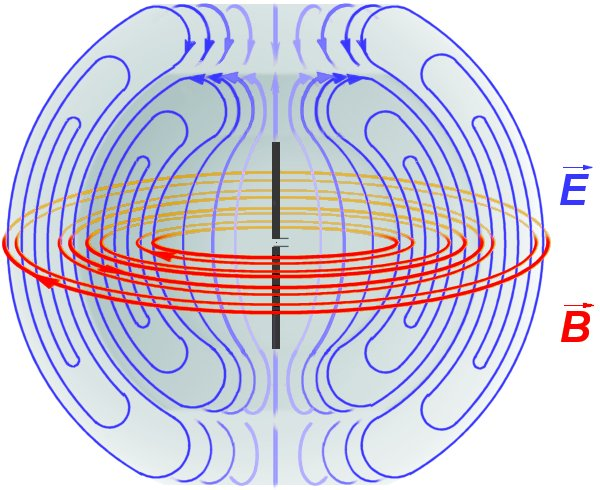
\includegraphics[width=0.33\textwidth]{./img/AntenaDipolar.jpg}
    \caption{Emisión radiativa de una antena dipolar. En azul ($\vec{E}$) se encuentra representado el campo eléctrico emitido, mientras que en rojo ($\vec{B}$) se muestra el campo magnético.}
    \label{fig:AntenaDipolar}
\end{figure}

\section{Teoría de Anisotropía}

La teoría de anisotropía puede explicarse fácilmente al considerar un único fluróforo. Por simplicidad consideremos que sus momentos de transición de excitación y emisión son colineales. La radiación de campo lejano emitida por el fluoróforo puede estudiarse mediante electrodinámica clásica y es análoga a un dipolo eléctrico (ver figura \ref{fig:AntenaDipolar}).

El campo eléctrico generado por un fluoróforo es

\begin{equation}
    E(\theta, \phi) = k \frac{\sin{ \theta}}{r} \hat{\theta},
\end{equation}

\noindent donde $k$ es la constante que determina la intensidad del dipolo eléctrico, $r$ la distancia al fluoróforo y se utilizó un sistema de coordenadas centrado en el fluoróforo cuyo eje z es compartido con la orientación del dipolo.

Por otro lado, si el dipolo no se encuentra alineado con el eje z, es fácil ver que la proyección del campo radiativo sobre el eje z será proporcional a $\cos{ \theta}$, mientras que sobre el eje x es proporcional a $\sin {\theta} \sin {\phi}$. Dichas proyecciones pueden apreciarse en la figura \ref{fig:RadiacionFluoroforo}.

\begin{figure}
    \centering
    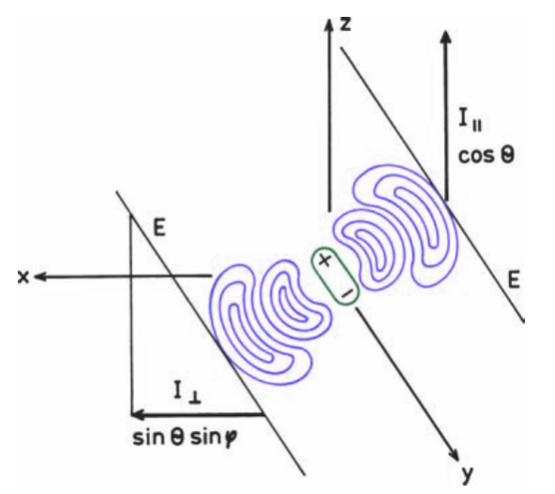
\includegraphics[width=0.4\textwidth]{./img/RadiacionFluoroforo.png}
    \caption{Emisión radiativa de un fluoróforo orientado al azar en un sistema de coordenadas esféricas. También se presentan las proyecciones en el eje z y eje x del campo irradiado\cite{Lakowicz2006}.}
    \label{fig:RadiacionFluoroforo}
\end{figure}

Una vez analizada la excitación y emisión de un único fluoróforo podemos comenzar a estudiar el comportamiento de un ensamble de estos ante la excitación con luz linealmente polarizada. Utilizando nuevamente argumentos de simetría, vemos que la probabilidad de excitar una molécula depende del ángulo $\theta$ que forma con el eje z, pero es independiente del ángulo $\phi$ que forma con el eje y. Luego, considerando que la intensidad de las proyecciones dependen

\begin{align}
    I_{\parallel} = & \cos^{2} \theta \label{eq:IntProyPar}\\
    I_{\perp}     = & \sin^{2} \phi \sin^{2} \theta, \label{eq:IntProyPerp}
\end{align}

\noindent y que podemos eliminar la dependencia con $\phi$ calculando el valor medio de $\sin^{2} \phi$ entre $0$ y $2\pi$, llegamos a

\begin{align}
    I_{\parallel} = & \cos^{2} \theta \label{eq:IntProyPar2}\\
    I_{\perp}     = & \frac{1}{2} \sin^{2} \theta. \label{eq:IntProyPerp2}
\end{align}

Analicemos ahora que sucede con la dependencia en $\theta$. Por generalidad, usaremos que $f(\theta) d\theta$ es la probabilidad de que una molécula se oriente entre $\theta$ y $\theta + d\theta$. Estimando las intensidades medidas a partir del promedio del ensamble apreciamos que

\begin{align}
    I_{\parallel} = & \int_0^{\pi/2} f(\theta) \cos^{2} \theta d\theta = k \langle \cos^{2} \theta \rangle \label{eq:IntProyPar3}\\
    I_{\perp}     = & \frac{1}{2} \int_0^{\pi/2} f(\theta) \sin^{2} \theta d\theta = \frac{k}{2} \langle \sin^{2} \theta \rangle. \label{eq:IntProyPerp3},
\end{align}

\noindent donde $k$ es una constante instrumental, que relaciona la intensidad del dipolo eléctrico con la ganancia de la cámara y otras características del sistema de detección. Reemplazando estas expresiones halladas en la ecuación \ref{eq:anisotropia} y utilizando identidades trigonométricas arribamos a

\begin{equation}
    r = \frac{3 \langle cos ^2 \theta \rangle - 1}{2}.
    \label{eq:anisotropiamedio}
\end{equation}

\noindent Cabe destacar que esta expresión es válida para ensambles con simetría alrededor del eje z. Además, entre las hipótesis utilizadas se planteó la colinealidad entre los momentos de transición de excitación y emisión, hecho que se cumple para muy pocas especies de fluoróforos pero que simplifica considerablemente los cálculos. Por último, se debe recalcar que $r$ se anula si el $\langle cos ^2 \theta \rangle = 1/3$, que, entre otros efectos, puede darse cuando el ángulo entre los momentos de excitación y emisión es de $54,7^{\circ}$. Este ángulo, llamado ángulo mágico también puede aprovecharse colocando el analizador horizontal $54,7^{\circ}$ respecto del vertical, y de esta forma se observa que $I_{\parallel} = 2 I_{\perp}$, ya que $\cos^{2} 54,7^{\circ} = 1/3$ y $\sin^{2} 54,7^{\circ} = 2/3$, resultando en que su suma sea proporcional a $I_{\parallel} + 2 I_{\perp}$. Esta disposición se utiliza para estudiar el decaimiento de intensidad de la muestra.

%En algunos casos, el objetivo es medir la intensidad total de fluorescencia y no la anisotropía de la muestra. Cuando este es el caso, los analizadores pueden colocarse de forma tal de obtener un valor proporcional a la intensidad total de fluorescencia independientemente de la anisotropía de la muestra. Si el analizador horizontal se ubica $54,7^{\circ}$ respecto del vertical, apreciamos que $I_{\parallel} = 2 I_{\perp}$, ya que $\cos^{2} 54,7^{\circ} = 1/3$ y $\sin^{2} 54,7^{\circ} = 2/3$, resultando en que su suma sea proporcional a $I_{\parallel} + 2 I_{\perp}$. Esta disposición se utiliza para estudiar el decaimiento de intensidad de la muestra.

A continuación, profundicemos sobre la dependencia de la distribución de probabilidad de los fluoróforos en $\theta$. Como se mencionó previamente, la probabilidad de excitar a un fluróforo es proporcional a $\cos^{2} \theta$, donde $\theta$ es el ángulo que el dipolo de excitación forma con el eje z (ver figura \ref{fig:FluoroforoExcitacion}). Además, el número de moléculas que forman un ángulo entre $\theta$ y $\theta + d\theta$ con el eje z es proporcional a $\sin{\theta} d\theta$, ya que se encuentran distribuidas completamente al azar. Combinando ambas estimaciones apreciamos que

\begin{equation}
    f(\theta) d\theta = \cos^{2} \theta \sin{ \theta} d\theta,
\end{equation}

\noindent resultando entonces en

\begin{equation}
    \langle \cos^{2} \theta \rangle = \frac{ \int_0^{\pi/2} f(\theta) \cos^{2} \theta d\theta} {\int_0^{\pi/2} f(\theta) d\theta} = \frac{3}{5}.
\end{equation}

\noindent Este último resultado aplicado a la ecuación \ref{eq:anisotropiamedio} implica una anisotropía máxima de $0,4$. Para llegar a este resultado se consideraron los dipolos de excitación y emisión como colineales, y no se tuvieron en cuenta efectos depolarizantes. Bajo estas condiciones se obtuvo $I_{\parallel} = 3 I_{\perp}$. Dado que esta es la anisotropía máxima que puede obtenerse de una muestra orientada al azar, cualquier valor medido superior es indicativo de artefactos en la observación\cite{Tramier2008}.

\begin{figure}
    \centering
    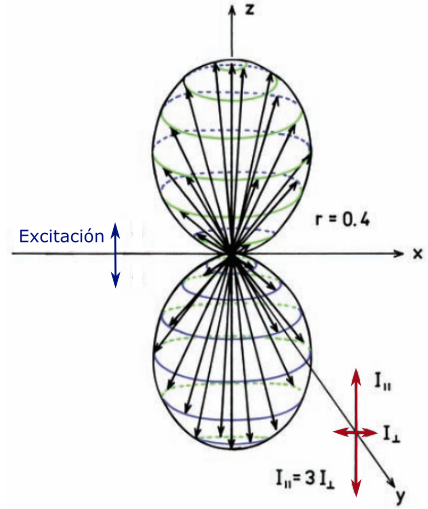
\includegraphics[width=0.4\textwidth]{./img/FluoroforoExcitacion.png}
    \caption{Distribución de fluoróforos excitados al utilizar luz linealmente polarizada en el eje z. Puede apreciarse la simetría del sistema alrededor de este eje\cite{Lakowicz2006}.}
    \label{fig:FluoroforoExcitacion}
\end{figure}

%\begin{figure}
%    \centering
%    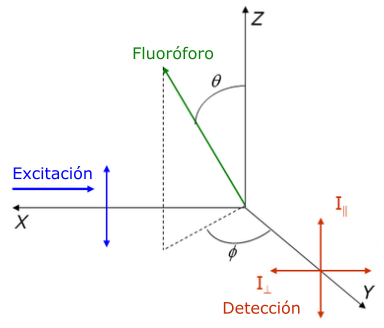
\includegraphics[width=0.4\textwidth]{./img/FluoroforoOrientado.png}
%    \caption{Proyecciones de un fluoróforo orientado al azar en el espacio\cite{Lakowicz2006}.}
%    \label{fig:FluoroforoOrientado}
%\end{figure}

Por último, es necesario recalcar que si en la muestra se encuentran más de una especie de fluoróforos, la anisotropía observada será

\begin{equation}
    r = \sum_i f_i r_i,
    \label{eq:anisotropiamezcla}
\end{equation}

\noindent donde $f_i$ es la fracción de intensidad de una especie, y $r_i$ su anisotropía\cite{Jablonski1960}. Esto resulta de considerar el carácter lineal de las intensidades emitidas por los fluoróforos, es decir,

\begin{equation}
    r = \frac{\sum_i I_i r_i}{\sum_i I_i}.
    \label{eq:anisotropiaInt}
\end{equation}


%%%%%%%%%%%%%%%%%%%%%%%%%%%%%%%%%%%%
\section{Métodos de Medición}

Los métodos de adquisición de datos para realizar análisis de anisotropía en polarización de fluorescencia se clasifican en formato de L ó T, según se utilicen uno o dos canales de emisión respectivamente. Estos métodos se aplican tanto a fluorímetros como a microscopios ópticos.


\begin{figure}
%    \begin{subfigure}{0.43\textwidth}
%            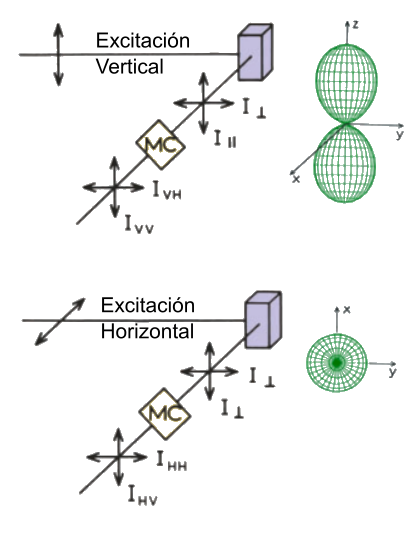
\includegraphics[width=0.99\textwidth]{./img/LFormat.png}
%            \caption{Esquema de la disposición en formato de L del sistema de adquisición. En esta disposición se adquieren los datos de ambas intensidades de manera secuencial.}
%            \label{fig:LFormat}
%    \end{subfigure}
%    ~
%    \begin{subfigure}{0.43\textwidth}
%        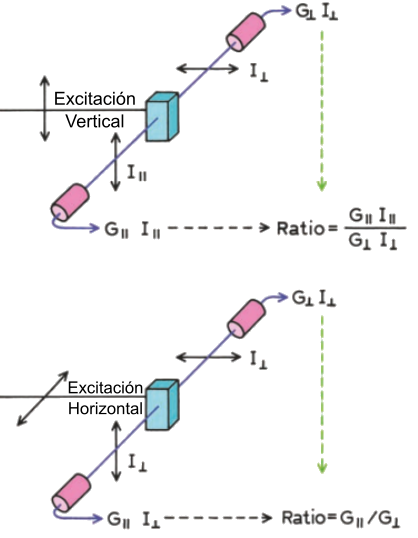
\includegraphics[width=0.99\textwidth]{./img/TFormat.png}
%        \caption{Esquema de la disposición en formato de T del sistema de adquisición. En esta disposición se adquieren datos de ambas intensidades simultáneamente.}
%        \label{fig:TFormat}
%    \end{subfigure}
    \centering
    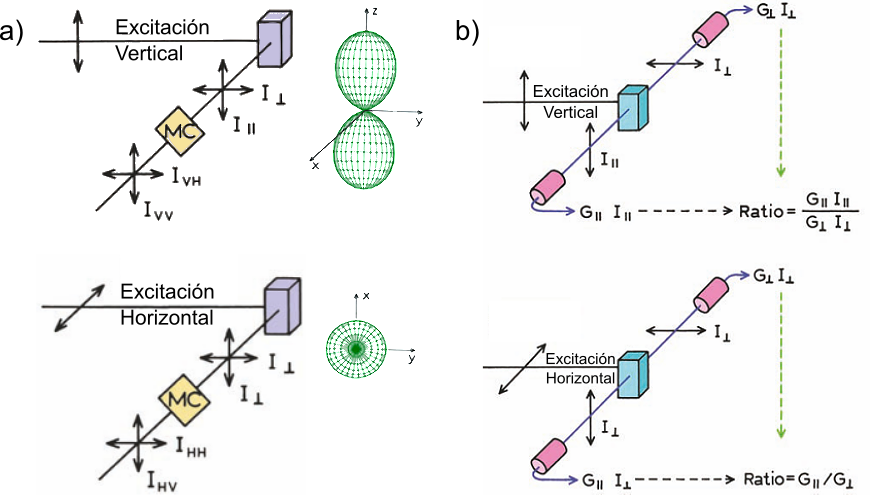
\includegraphics[width=0.9\textwidth]{./img/Formats.png}
    \caption{Disposiciones experimentales utilizadas para adquisición de datos en anisotropía de fluorescencia\cite{Lakowicz2006}. \textbf{a)}: Esquema de la disposición en formato de L del sistema de adquisición. En esta disposición se adquieren los datos de ambas intensidades de manera secuencial. \textbf{b)}: Esquema de la disposición en formato de T del sistema de adquisición. En esta disposición se adquieren datos de ambas intensidades simultáneamente.}
    \label{fig:Formats}
\end{figure}

\subsection{Formato de L o de Canal Único}

La disposición en forma de L es la más utilizada comúnmente ya que se necesita un único canal de emisión. Consiste en incidir sobre la muestra con luz linealmente polarizada y observar su emisión por medio de un monocromador y un analizador, como se muestra en la figura \ref{fig:Formats}a.

Desde el punto de vista experimental, la sensibilidad del sistema para observar intensidad de fluorescencia en ambos ejes puede ser distinta. Dado que el objetivo es obtener mediciones de $I_{\parallel}$ e $I_{\perp}$, procedemos a calcularlos a partir de las observaciones realizadas. En primer lugar, tenemos acceso a las intensidades cruzadas que son proporcionales a las intensidades buscadas de la forma

\begin{align}
    I_{VV} =& k S_V I_{\parallel} \\
    I_{VH} =& k S_H I_{\perp},
\end{align}

\noindent donde $k$ es una constante instrumental y $S_V$ y $S_H$ las sensibilidades de ambas disposiciones del analizador. El subíndice de las intensidades observadas corresponden: el primero a la orientación del eje de polarización del haz de excitación y el segundo al de emisión observado, siendo $V$ vertical, y $H$ horizontal.

Puede apreciarse rápidamente que la relación entre ambas intensidades nos devuelve

\begin{equation}
    \frac{I_{VV}}{I_{VH}} = \frac{S_V}{S_H} \frac{I_{\parallel}}{I_{\perp}} = G \frac{I_{\parallel}}{I_{\perp}},
\end{equation}

\noindent donde $G$ corresponde a cuanto más sensible es un canal respecto del otro, es decir, da cuenta de las depolarizaciones introducidas por el sistema óptico en cuestión y no por la muestra. Se debe notar que es necesario conocer el valor de $G$ para obtener las intensidades buscadas. Con este objetivo en mente, es fácil mostrar que utilizando una haz de excitación polarizado horizontalmente hallamos

\begin{equation}
    \frac{I_{HV}}{I_{HH}} = \frac{S_V}{S_H} \frac{I_{\perp}}{I_{\perp}} = G,
\end{equation}

\noindent ya que al rotar el eje de polarización de la excitación, se rota también el la distribución de los estados excitados de forma tal que en la observación solo se observan las $I_{\perp}$, como se muestra en la figura \ref{fig:Formats}a.

La anisotropía de la muestra se puede calcular a partir de las observaciones realizadas utilizando

\begin{equation}
    \frac{I_{VV}}{I_{VH} G} = \frac{I_{VV}}{I_{VH}} \frac{I_{HV}}{I_{HH}} = \frac{I_{\parallel}}{I_{\perp}},
\end{equation}

\noindent y, por lo tanto,

\begin{equation}
    r = \frac{I_{\parallel}/I_{\perp} - 1}{I_{\parallel}/I_{\perp} +2},
    \label{eq:r1}
\end{equation}

\noindent que es análogo a

\begin{equation}
    r = \frac{I_{VV}-GI_{VH}}{I_{VV}+2GI_{VH}}.
    \label{eq:r2}
\end{equation}

\subsection{Formato de T o de Dos Canales}

En la disposición en forma de T se utilizan dos canales de emisión para adquirir los valores de intensidad de fluorescencia simultáneamente. En esta disposición, los polarizadores de emisión no se rotan durante la medición y, por lo tanto, no cambia su sensibilidad. Además, la velocidad de adquisición de datos es mayor ya que se observan ambos canales al mismo tiempo.

De manera análoga a la disposición en forma de L, se obtienen los relaciones entre las intensidades medidas, $R_V$ y $R_H$

\begin{align}
    R_V =& \frac{G_{\parallel} I_{\parallel}}{G_{\perp} I_{\perp}} \\
    R_H =& \frac{G_{\parallel}}{G_{\perp}},
\end{align}

\noindent donde $G_{\parallel}$ and $G_{\perp}$ son las sensibilidades correspondientes a cada canal. Por último, calculando la relación entre ambas llegamos a

\begin{equation}
    \frac{R_V}{R_H} = \frac{I_{\parallel}}{I_{\perp}},
\end{equation}

\noindent expresión que podemos combinar con las ecuaciones \ref{eq:r1} y \ref{eq:r2} para calcular la anisotropía buscada. Se debe recalcar que esta metodología tiene dificultades cuando alguna de las intensidades de fluorescencia es muy baja.

\subsection{Implementación en Microscopía}

Es posible implementar en un microscopio óptico común un arreglo de polarizadores que permita obtener información sobre la anisotropía en la polarización de fluorescencia. Estos sistemas, denominados microscopios de imágenes de anisotropía de fluorescencia, permiten obtener mapas de anisotropía de diversas muestras.

\begin{figure}
    \centering
    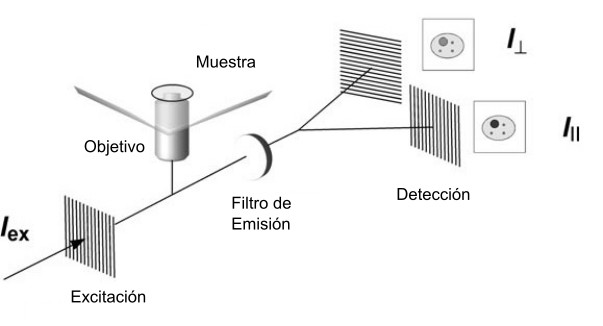
\includegraphics[width=0.6\textwidth]{./img/EsquemaAnisotropia.png}
    \caption{Esquema del armado experimental utilizado para observar anisotropía en microscopía óptica. Se aprecia que el canal de excitación y emisión es el mismo y se utiliza un espejo dicroico para separar ambas señales\cite{Chan2011}.}
    \label{fig:EsquemaMicro}
\end{figure}

La implementación de anisotropía de fluorescencia en microscopía puede clasificarse también según se utilicen uno o dos canales de emisión. Las adaptaciones incluyen un polarizador entre la fuente y la muestra, y otro entre la muestra y la cámara de adquisición, como se muestra en la figura \ref{fig:EsquemaMicro}. En algunos casos, se utilizan cristales birefringentes (por ejemplo: calcita) para separar las componentes paralela y perpendicular de la emisión, y visualizarlas al mismo tiempo mediante la cámara\cite{Yao2010}.

La cuantificación de anisotropía de fluorescencia en microscopía presenta varios desafíos. Muchos de los componentes presentes en un microscopio inducen depolarización de la luz que si no es corregida adecuadamente conlleva a errores sistemáticos\cite{Chan2011}. En primer lugar, las lentes objetivo utilizadas comúnmente tienen amplitud numérica elevada. Esto último genera una mezcla de distintas polarizaciones ya que los conos de luz de excitación y emisión son subtendidos en un amplio ángulo sólido en el punto de muestreo (ver figura \ref{fig:NA})\cite{Andreev1993}.

\begin{figure}
    \centering
    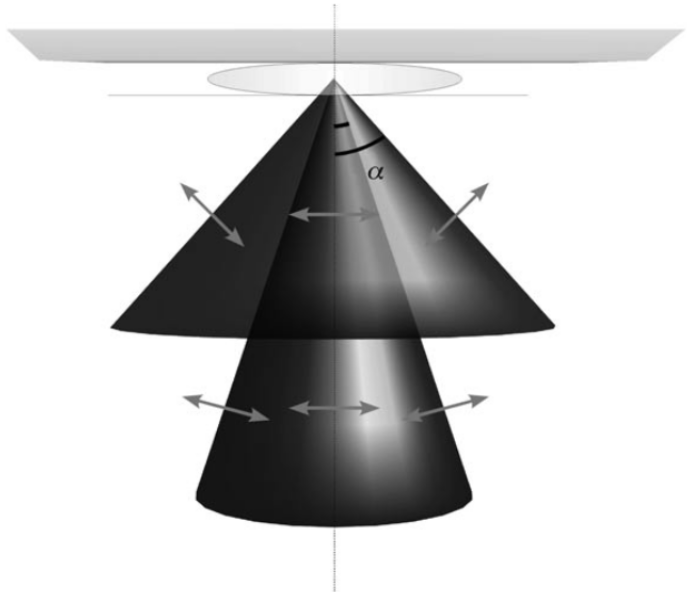
\includegraphics[width=0.4\textwidth]{./img/NA.png}
    \caption{Depolarización producida por lentes objetivo con amplitud numérica alta. El cono de luz en el punte de observación tiene un ángulo sólido mayor para lentes con apertura numérica más grande, mezclando las polarizaciones verticales con las horizontales\cite{Chan2011}.}
    \label{fig:NA}
\end{figure}

Por otro lado, se debe destacar que la disposición de los haces de luz de excitación y emisión no permiten clasificar al sistema en las disposiciones descriptas previamente. En este caso, el camino óptico del haz de excitación es el mismo que el de emisión. Esto último vuelve inviable la posibilidad de medir $I_{\perp}$ en ambos ejes de polarización, obligando a utilizar un valor de anisotropía de referencia para calibrar el sistema.

Con el objetivo de corregir las posibles depolarizaciones generadas por el sistema óptico del microscopio, se pueden comparar las anisotropias observadas mediante microscopía con las obtenidas por medio de un fluorímetro comercial. Simultáneamente, se requiere la calibración del factor G que tiene en cuenta las diferencias en sensibilidad del sistema para polarizaciones cruzadas. El factor G puede hallarse a partir de un valor de referencia de anisotropía de un fluoróforo utilizando la ecuación

\begin{equation}
    G = \frac{I_{\parallel} (1 - r_{ref})}{I_{\perp} (1 + 2r_{ref})},
\end{equation}

\noindent donde $r_{ref}$ es el valor de anisotropía conocido de la muestra. Dado que el factor G es dependiente de la longitud de onda utilizada, se debe calibrar para el rango utilizado en el experimento.



%%%%%%%%%%%%%%%%%%%%%%%%%%%%%%%%%%%%
\section{Factores Depolarizantes}

Con el objetivo de aprovechar al máximo las ventajas que proveen las técnicas de anisotropía de fluorescencia, debemos conocer primero las fuentes de depolarización. Estas pueden provenir de características intrínsecas al fluoróforo, como es el desplazamiento angular que existe entre el dipolo de excitación y el de emisión, así como también por causas extrínsecas, como son la difusión rotacional y la transferencia de energía de resonancia\cite{Lakowicz2006}.

El carácter dipolar del fluoróforo nos permite estudiar la orientación de estructuras subcelulares. El desplazamiento angular entre el dipolo de excitación y el de emisión nos introduce una depolarización que debe ser tenida en cuenta a la hora de estudiar dichas orientaciones. En la figura \ref{fig:GFPDipole} se presentan imágenes de cristales de proteína verde fluorescente donde se aprecian las distintas intensidades de fluorescencia en las distintas polarizaciones. Estudiar las intensidades emitidas mientras se rotan los polarizadores de excitación y emisión permiten detectar los ejes de ambos dipolos\cite{Inoue2002}.

\begin{figure}
    \centering
    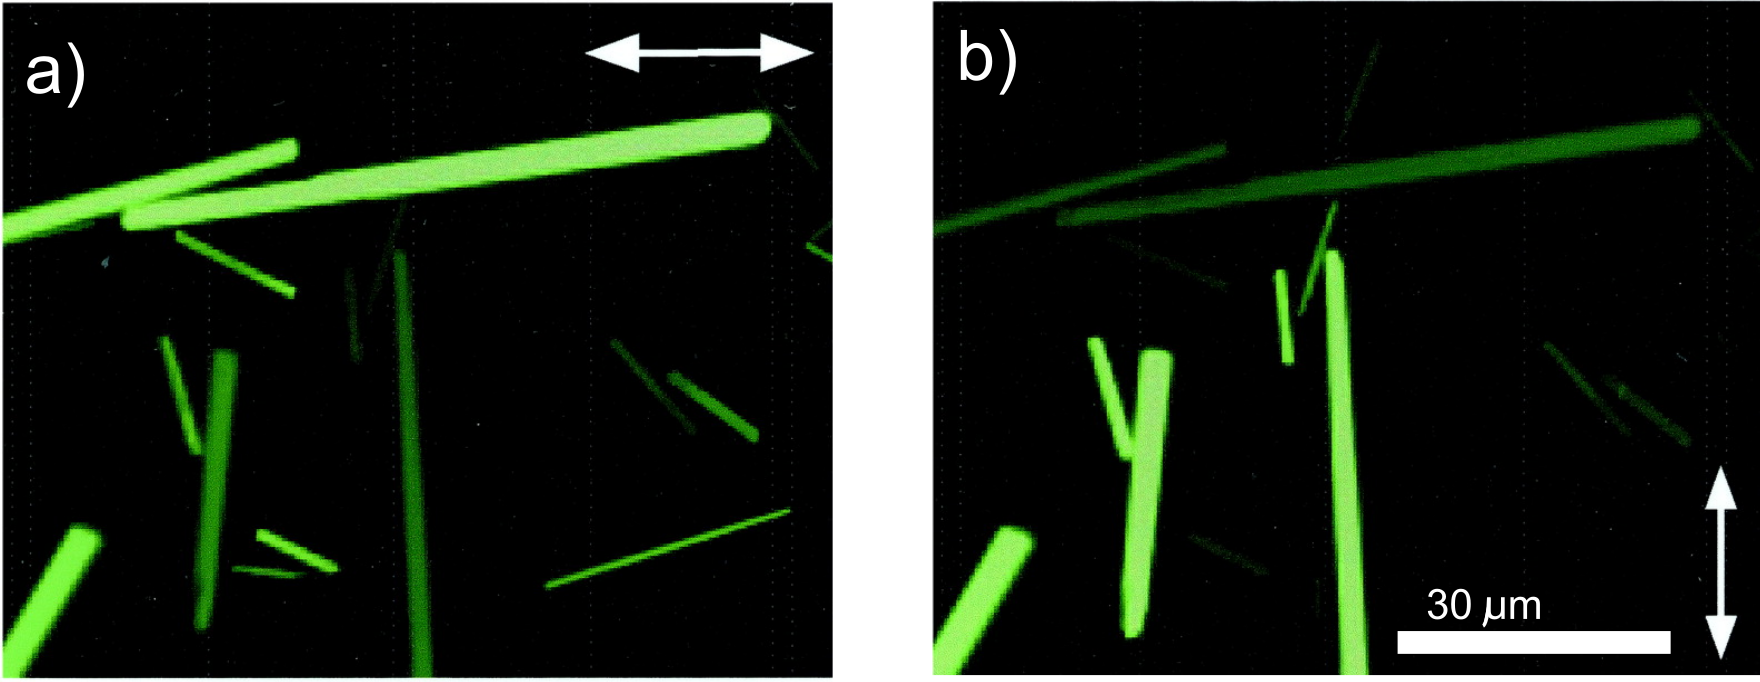
\includegraphics[width=0.8\textwidth]{./img/GFPDipole.png}
    \caption{Cristales de proteínas verde fluorescente\cite{Inoue2002}. Se excitaron las muestras con luz linealmente polarizada en ambos casos (orientada según las flechas) y no se utilizó analizador en ningún caso.}
    \label{fig:GFPDipole}
\end{figure}

Estudiar la orientación del fluoróforo unido a la cabeza de myosina (S$_1$) permitió identificar su disposición y orientación al unirse a F-actina. En el trabajo de \textit{Borejdo et al.}\cite{Andreev1993}, se concluyó que S$_1$ podía unirse de dos formas distintas según se halle en exceso o déficit en relación a la cantidad de F-actina.

La difusión rotacional es producto de las rotaciones del fluoróforo mientras este se encuentra en el estado excitado. Su efecto sobre la anisotropía surge a partir del juego entre el tiempo de vida de fluorescencia y el tiempo de correlación de rotación. Entre los factores que afectan el tiempo de correlación de rotación se encuentran la viscosidad del medio en que se halla disuelto el fluoróforo, el tamaño de este, y si se encuentra unido a otras moléculas (ver figura \ref{fig:DifusionRotacional}). 

\begin{figure}
    \centering
    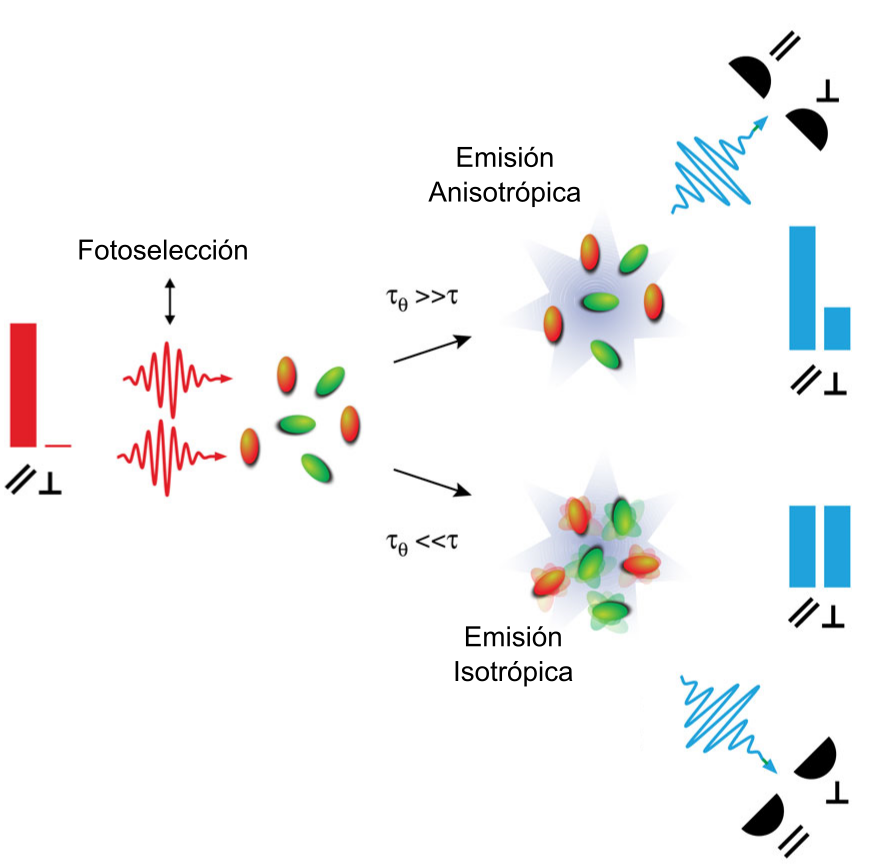
\includegraphics[width=0.6\textwidth]{./img/DifusionRotacional.png}
    \caption{Esquema del efecto que tiene la difusión rotacional sobre la anisotropía de fluorescencia. Se realiza una fotoselección incidiendo con luz linealmente polarizada y se observa una emisión anisotrópica cuando el tiempo de correlación de rotación es considerablemente mayor al de vida media de la fluorescencia, o emisión isotrópica si la situación es la inversa\cite{Dubach2014}}
    \label{fig:DifusionRotacional}
\end{figure}

Conociendo el efecto que tiene la viscosidad del medio sobre el tiempo de correlación de rotación del fluoróforo, la anisotropía de fluorescencia puede ser utilizada para obtener información sobre parámetros reológicos del citosol, como se muestra en el trabajo de \textit{Verkman et al.}\cite{Swaminathan1997}. Por otro lado, dado que la unión del fluoróforo a otra molécula produce un cambio en la anisotropía, se la puede utilizar para reportar la proporción de fluoróforos ligados entre el total de fluoróforos. La ecuación \ref{eq:anisotropiamezcla} y conocer los valores específicos de anisotropía de cada estado permiten hallar esta proporción. \textit{Weissleder et al.}\cite{Dubach2014} utilizan esta técnica \textit{in vivo} para observar la dinámica de interacción entre la droga y su blanco (Olaparib) en tiempo real, mostrando su utilidad para descifrar la dinámica intracelular.

%Por último, otros factores que producen depolarización son la transferencia de energía de resonancia y la dispersión. La transferencia de energía de resonancia se produce en soluciones muy concentradas, en estas la distancia entre fluoróforos es comparable a la distancia característica $R_0$. Estas concentraciones generalmente son considerablemente mayores a las utilizadas normalmente, del orden miliMolar. Por otro lado, algunas muestras biológicas pueden ser turbias produciendo dispersión de fotones que afectan de forma distinta la anisotropía según se produzca antes o después de excitar al fluoróforo.

%%%%%%%%%%%%%%%%%%%%%%%%%%%%%%%%%
\section{Transferencia de Energía de Resonancia de Förster}

Cuando dos fluoróforos se encuentran próximos entre si, la energía de radiación puede ser transferida de forma no radiativa de uno a otro como resultado de acoplamiento dipolo-dipolo\cite{GreccoBastiaens2009}. Este fenómeno, denominado transferencia de energía de resonancia de Förster (FRET), puede ser explicado mediante electrodinámica clásica. La utilización generalizada de FRET se debe a que la distancia característica de esta transferencia es típicamente del orden del tamaño de una proteína o grosor de la membrana plasmática, hecho que lo vuelve valioso para estudiar colocalización e interacción molecular en escalas inferiores a la resolución del microscopio, así como también actividad enzimática\cite{Lakowicz2006}.

La transferencia de energía ocurre entre una molécula donante en el estado excitado y una aceptora en el estado fundamental. Las moléculas donante tienen menor longitud de onda de emisión y en general se solapa con la de excitación de la aceptora, como se muestra en la figura \ref{fig:EspectroFRET}\cite{Lakowicz2006}. La eficiencia del flujo de energía se define como

\begin{equation}
    E = \frac{1}{1+ \left( r/R_0 \right)^6},
\end{equation}

\noindent donde $r$ es la separación entre fluoróforos y $R_0$ es la distancia a la cual la mitad de la energía de excitación es transferida. Notar que si la concentración de fluoróforos es del orden miliMolar, la separación entre estos es del orden de $R_0$.

La separación $R_0$ puede ser calculada teóricamente a partir de la tasa de transferencia de energía de resonancia. Realizando los cálculos correspondientes se llega a que $R_0$ medido en \AA es

\begin{equation}
    R_0=(\kappa^2 \times J(\lambda) \times n^{-4} \times Q_D)^{1/6}\times 9.78 \times 10^3,
\end{equation}

\noindent donde $\kappa$ es la orientación relativa de los dipolos de ambos fluoróforos, $J(\lambda)$ es el solapamiento en los espectros de emisión y excitación del donante y aceptor (ver figura \ref{fig:EspectroFRET}), $n$ es el índice de refracción del medio y $Q_D$ es el rendimiento cuántico del dador\cite{Lakowicz2006}.

Hasta ahora hemos considerado la transferencia de energía entre dos fluoróforos distintos, denominado heteroFRET, pero esta puede ocurrir entre fluoróforos del mismo tipo si los espectros de emisión y excitación se superponen. Este caso, denominado homoFRET, se caracteriza por tener corrimiento en longitud de onda de Stokes suficientemente pequeños y elevados coeficientes de extinción (ver figura \ref{fig:EspectroFRET}b, propiedades que culminan en separaciones $R_0$ de alrededor de 57\AA\cite{Lakowicz2006}. En este caso, se analizan los cambios en la anisotropía de la muestra en lugar de la transferencia de energía entre distintos canales espectrales. En el trabajo de \textit{Stegemann et al.} se utiliza un sensor basado en homoFRET que es clivado por la caspasa-3 activa. Este se utiliza para estudiar la inicialización de apoptosis en respuesta a especies reactivas del oxígeno generadas mediante superficies fotofuncionales\cite{Grecco2015}.

\begin{figure}
\centering
    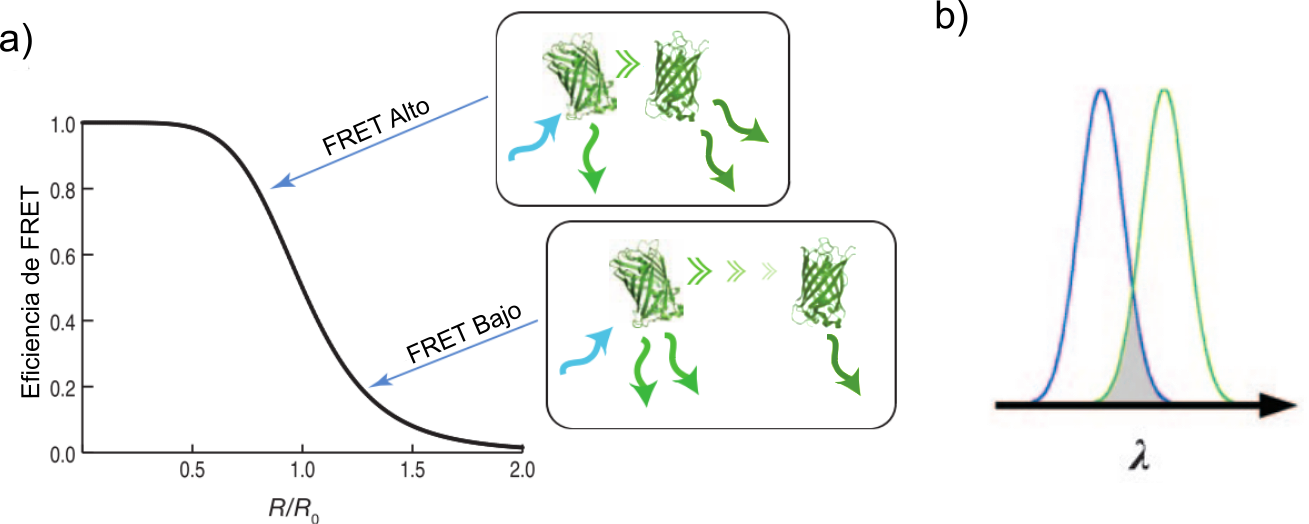
\includegraphics[width=0.8\textwidth]{./img/FRETAnisotropia.png}
    \caption{La Eficiencia de FRET depende de varios factores. \textbf{a)} Se muestra la eficiencia de FRET en función de la separación de fluoróforos. $R_0$ es la separación a la cual la eficiencia se reduce a la mitad. \textbf{b)} La superposición entre los espectros de emisión y el de excitación permiten que haya FRET entre ambos fluoróforos idénticos.}
    \label{fig:EspectroFRET}
\end{figure}

Entre las ventajas que presenta homoFRET respecto de heteroFRET se encuentra que la utilización de un único tipo de fluoróforo por sensor permite reducir el ancho espectral ocupado por cada sensor y así colocar más tipos de reporteros en cada célula. Análogamente, es posible utilizar fluoróforos distintos cuyo espectro sea suficientemente similar como para que ocurre homoFRET entre ambos, o mejor dicho seudo-homoFRET. Seleccionar cuidadosamente la pareja de fluoróforos es crucial para que el sensor confeccionado sea óptimo.

%En particular, se utilizaron biosensores que consistían en dos fluoróforos unidos por secuencias específicas de aminoácidos que son seccionadas por las caspasas, cuya actividad enzimática se desea estudiar. Con el objetivo de reportar la actividad de ambas vías iniciadoras, intrínseca y extrínseca, así como también la actividad de la caspasa efectora se utilizaron tres biosensores distintos de homoFRET. La ventaja que presenta este método respecto de heteroFRET es que la utilización de un único tipo de fluoróforo por sensor permite reducir el ancho espectral ocupado por cada sensor y así colocar más tipos de reporteros en cada célula.

%Los pares de fluoróforos utilizados fueron mCitrine-mCitrine, mCerulean-tagBFP y mKate2-mCherry. Es importante recalcar que los últimos dos pares, aunque están conformados por fluoróforos distintos, sus espectros son tan similares que no pueden ser diferenciados fácilmente y por esa razón se estudian mediante homoFRET.


%%%%%%%%%%%%%%%%%%%%%%%%%%%%%%%%%%%
\section{Análisis de Anisotropía en la Polarización}

Habiendo visto los conceptos teóricos, podemos estudiar como obtener información del estado del ensamble de fluoróforos a partir de la anisotropía observada. Comencemos por analizar un único par de fluoróforos distintos optimizados para homoFRET. La anisotropía observada puede hallarse mediante la ecuación \ref{eq:anisotropiaInt}

\begin{equation}
r = \frac{\sum_i I_i r_i}{\sum_i I_i}, \tag{\ref{eq:anisotropiaInt}}
\end{equation}

\noindent donde esta es el promedio pesado por las intensidades correspondientes al sensor en estado dimérico y monomérico de las anisotropías respectivas. 

Por otro lado, es importante notar que la intensidad observada de un fluoróforo en estado monomérico no será la misma que cuando este en estado dimérico. Dado que los distintos fluoróforos poseen propiedades fotofísicas diferentes, como sus espectros de absorción y emisión, su rendimiento cuántico, entre otras, sus brillos por molécula detectados serán diferentes. Luego, cuando estas se hallan en forma dimérica y ocurre FRET entre ellas, las intensidades observadas son distintas a cuando se hayan por separado ya que al trasmitirse energía entre ellas, los canales de detección detectarán intensidades distintas. Por otro lado, aunque se trate la misma especie de fluoróforo, la maduración de este puede no ser igual para ambos monómeros constituyentes, presentando el mismo fenómeno. De esta forma, las intensidades del sensor en cada estado pueden expresarse como


\begin{align}
    I_M &= b_M M\\
    I_D &= b_D 2D,
\end{align}

\noindent siendo $b_D$ y $b_M$ los brillos de un monómero de fluoróforo unido a otro o separado, respectivamente. $M$ y $D$ son las concentraciones de monómeros y dímeros, mientras que $I_M$ e $I_D$ dan cuenta de su intensidad.

En una primera aproximación al problema, podemos hacer el experimento mental de considerar distintas cubetas con variadas concentraciones, relativas y totales, de un tipo de sensor en sus distintos estados. Por simplicidad, podemos darle un orden temporal a las cubetas, que posteriormente nos ayudará a comprender lo que sucede dentro del sistema biológico.

Luego, supongamos que se tiene una única cubeta con una cantidad fija de sensores. Dado que la cantidad de monómeros es constante, podemos afirmar

\begin{equation}
    C = M + 2D,
    \label{eq:C_cte}
\end{equation}

\noindent hecho que nos permitirá expresar todo en función de la proporción de fluoróforo en estado monomérico ($m=M/C$). Es así que la ecuación \ref{eq:anisotropiaInt} puede reescribirse como

\begin{equation}
    r = \frac{I_M r_M + I_D r_D}{I_M+I_D} = \frac{b_M M r_M + b_D 2D r_D}{b_M M+b_D 2D} = \frac{m r_M + b (1-m) r_D}{m+b (1-m)},
    \label{eq:AnisotropiaFromParams}
\end{equation}

\noindent donde se tomó factor común $b_M C$ en el numerador y denominador, y se uso que $2D = C - M$. Las anisotropías correspondientes a los estados monoméricos y diméricos se denominaron $r_M$ y $r_D$, respectivamente. Por otro lado, $b = b_D/b_M$ representa la relación entre el brillo del monómero en cada estado y $m$ es la proporción de fluoróforo en estado monomérico, por lo que se encuentra entre $0$ y $1$. La expresión hallada nos permite vincular la anisotropía medida con la proporción de fluoróforo en cada estado.

A continuación, supongamos que en algún momento se desencadena una reacción enzimática que comienza a clivar y separar los dímeros en sus monómeros constitutivos. De esta forma, la curva de proporción de monómero respecto a la cantidad total de fluoróforo tendrá una forma sigmoidea o boltzmanniana como se muestra en la figura \ref{fig:m_sim}. El momento en que comienza la reacción, así como su tasa, son parámetros que definen distintas curvas y serán elegidos arbitrariamente por ahora. Además, la proporción de fluoróforo inicial en estado dimérico, como la proporción de monómeros al final de la reacción también deben ser determinados arbitrariamente, en particular, asumamos que iniciamos el experimento con todo el fluoróforo disponible en estado dimérico, pero culminamos la reacción con solo el 80$\%$ del fluoróforo en estado monomérico.

\begin{figure}
\centering
    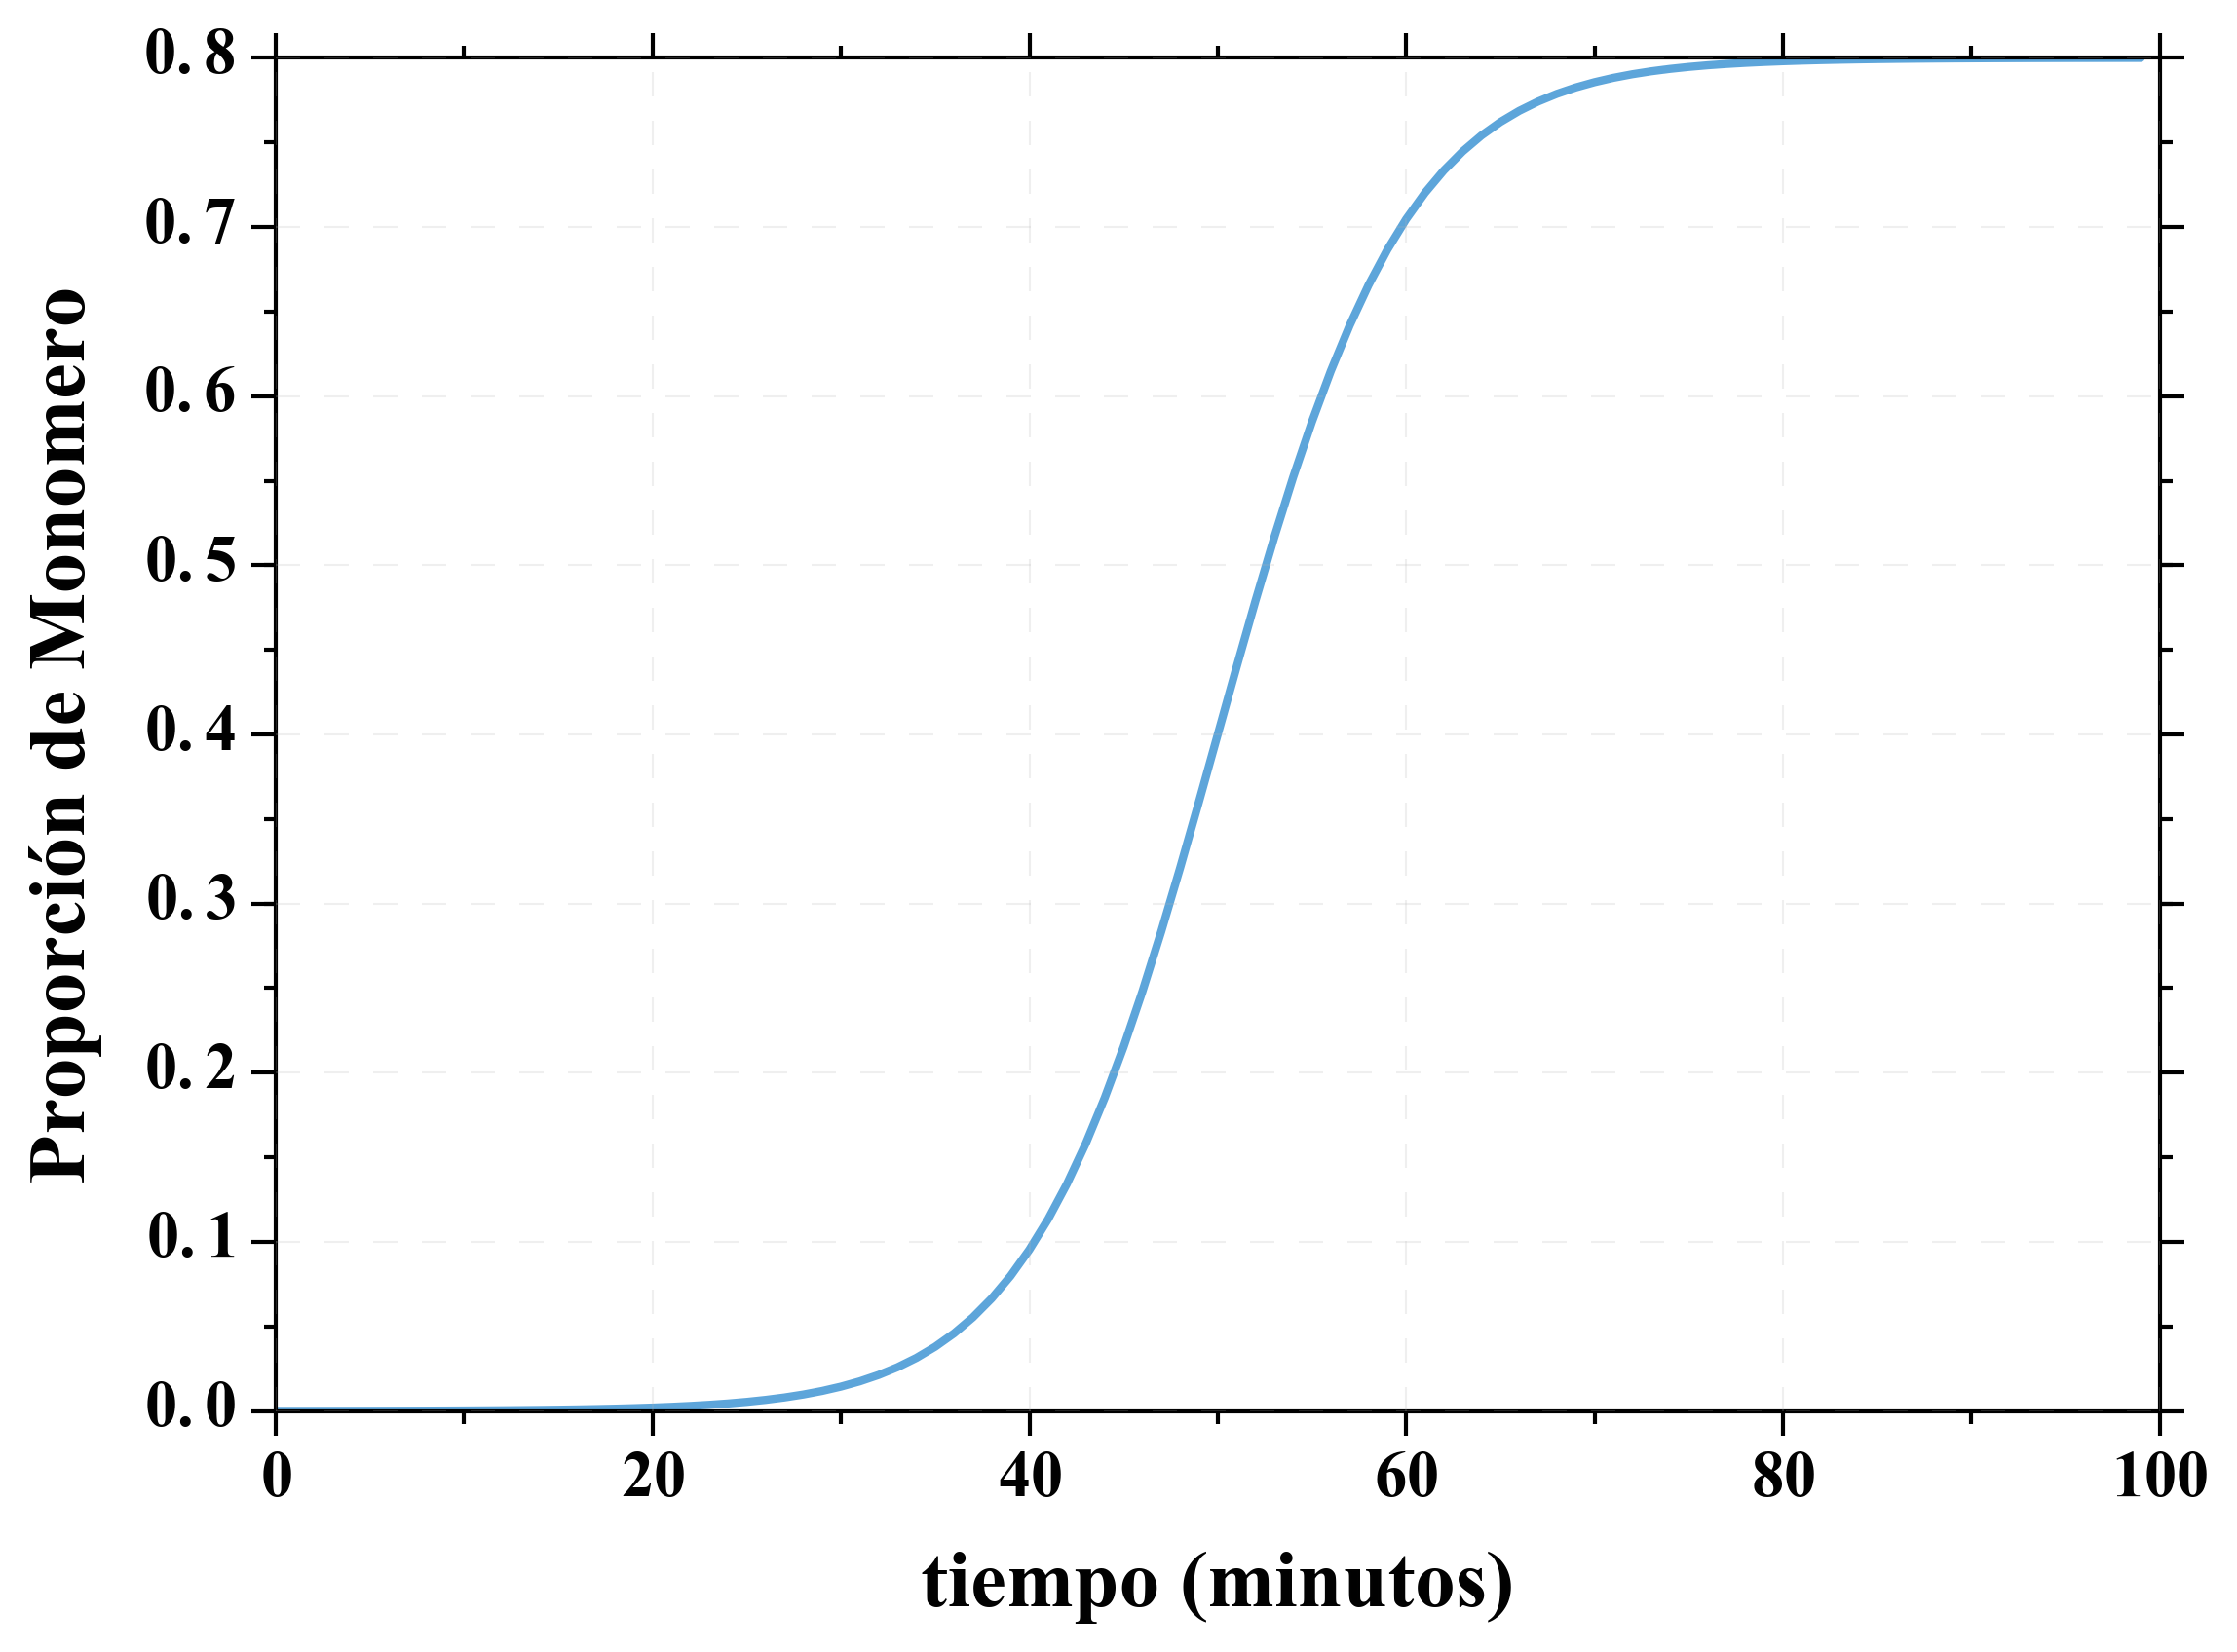
\includegraphics[width=0.6\textwidth]{./img/m_sim.png}
    \caption{Curva típica de variación de la proporción de sensores en estado monomérico simulada. Se determinó arbitrariamente que previo a la reacción todo el sensor se halle en estado monomérico, mientras que al final solo el $80\%$ se halla clivado.}
    \label{fig:m_sim}
\end{figure}

Si conocemos la proporción de fluoróforos en cada estado para cada cubeta, o mejor dicho, para cada tiempo, podemos calcular la anisotropía utilizando la ecuación \ref{eq:AnisotropiaFromParams}. Además de la proporción, es necesario conocer las anisotropías correspondientes a cada estado, así como también la relación entre brillos ($b$) para poder realizar el cálculo. Utilizando $m(t)$ simulado previamente y asumiendo que se trata del sensor de mCitrine-mCitrine, cuyas anisotropías teóricas son $r_D=0.221$ y $r_M=0.303$, se confeccionaron las distintas curvas de anisotropía. Por último, se realizó un barrido en el valor de $b$ desde $0.2$ a $0.8$ para confeccionar la figura \ref{fig:aniso_sim}. Se seleccionó este rango de valores de $b$ ya que se sabe experimentalmente que $b_M>b_D$, por lo que $0<b<1$. Se debe recalcar como el valor de $b$ cambia levemente la pendiente, así como el máximo valor de anisotropía alcanzado.

\begin{figure}
\centering
    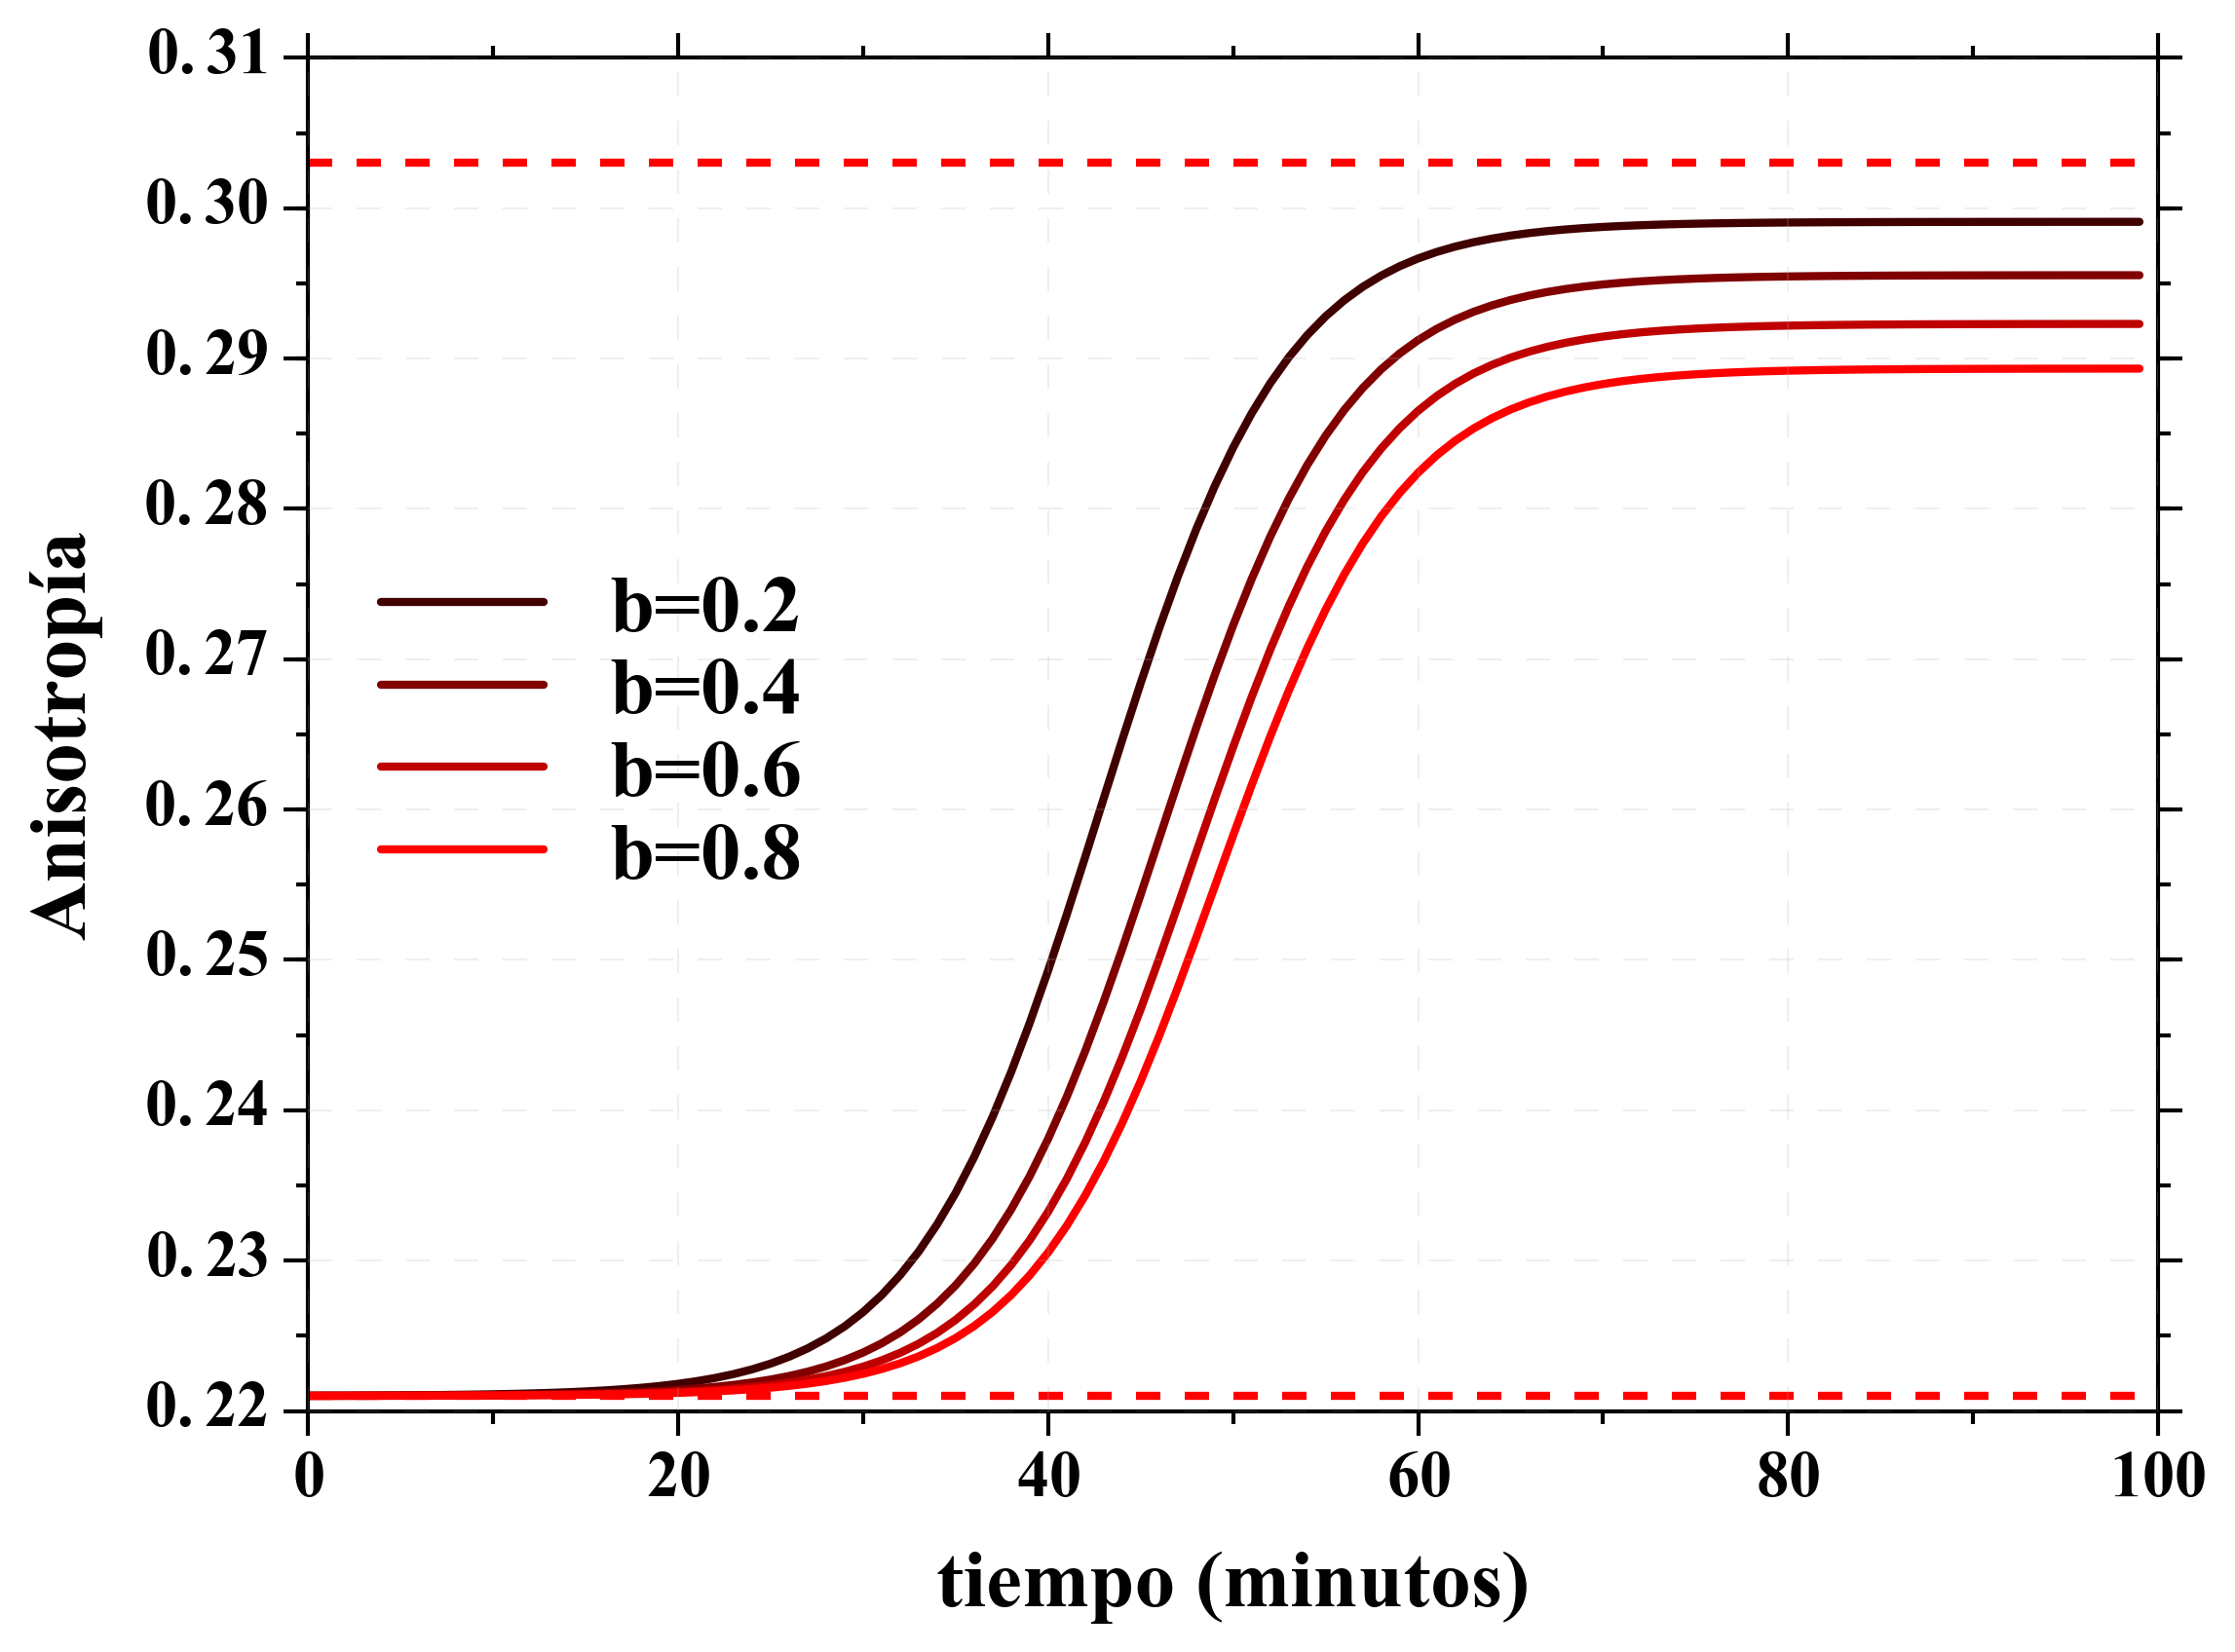
\includegraphics[width=0.6\textwidth]{./img/r_sim.png}
    \caption{Curva de anisotropía generada a partir de la curva simulada para $m$ considerando al fluróforo en cuestión como mCitrine. Se utilizaron $r_D=0.221$ y $r_M=0.303$, mientras que para el valor de $b$ se realizó un barrido entre $0.2$ y $0.8$. Las anisotropías del monómero y dímero se graficaron para remarcar los máximos y mínimos de anisotropía observabeles.}
    \label{fig:aniso_sim}
\end{figure}

Es interesante notar en la figura \ref{fig:aniso_sim} la relación entre los parámetros $b$ y $r_D$, ya que vemos que disminuir $b$ aumenta el máximo de anisotropía alcanzado cuando se cliva el $80\%$ del sensor. Esto quiere decir que podría disminuir $r_D$ o variar la proporción máxima clivada para obtener la misma curva. Esta relación entre parámetros complica el análisis a la hora de ajustar curvas ya que más de una combinación de parámetros devuelven curvas muy similares. Además, se aprecia que cuando no todo el fluoróforo es clivado, el hecho de utilizar fluoróforos distintos nos permite mejorar el rango dinámico del sensor.

Por otro lado, sabiendo que el brillo del fluoróforo es distinto en cada estado, podemos estudiar la fluorescencia total emitida para obtener información sobre el valor de $b$. Sin ir más lejos, el denominador en la ecuación \ref{eq:AnisotropiaFromParams} es igual a la intensidad total de fluorescencia emitida, es decir,

\begin{equation}
    I_T = I_M+I_D = b_M M+b_D 2D = b_M C (m+b (1-m)), \label{eq:Int_fromFit}
\end{equation}

\noindent donde $b_M C$ sirve de factor escala y representa la intensidad máxima de fluorescencia que puede alcanzarse si todo el sensor es clivado. Esto hecho puede verificarse viendo que si $m=1$, $I_T=b_M C$, sumado al hecho de que C representa la cantidad total de fluoróforo y $b_M$ es el brillo del fluoróforo en estado monomérico. Se grafican en la figura \ref{fig:f_sim} las curvas de fluorescencia total observada para el barrido en $b$ confeccionado previamente.

\begin{figure}
\centering
    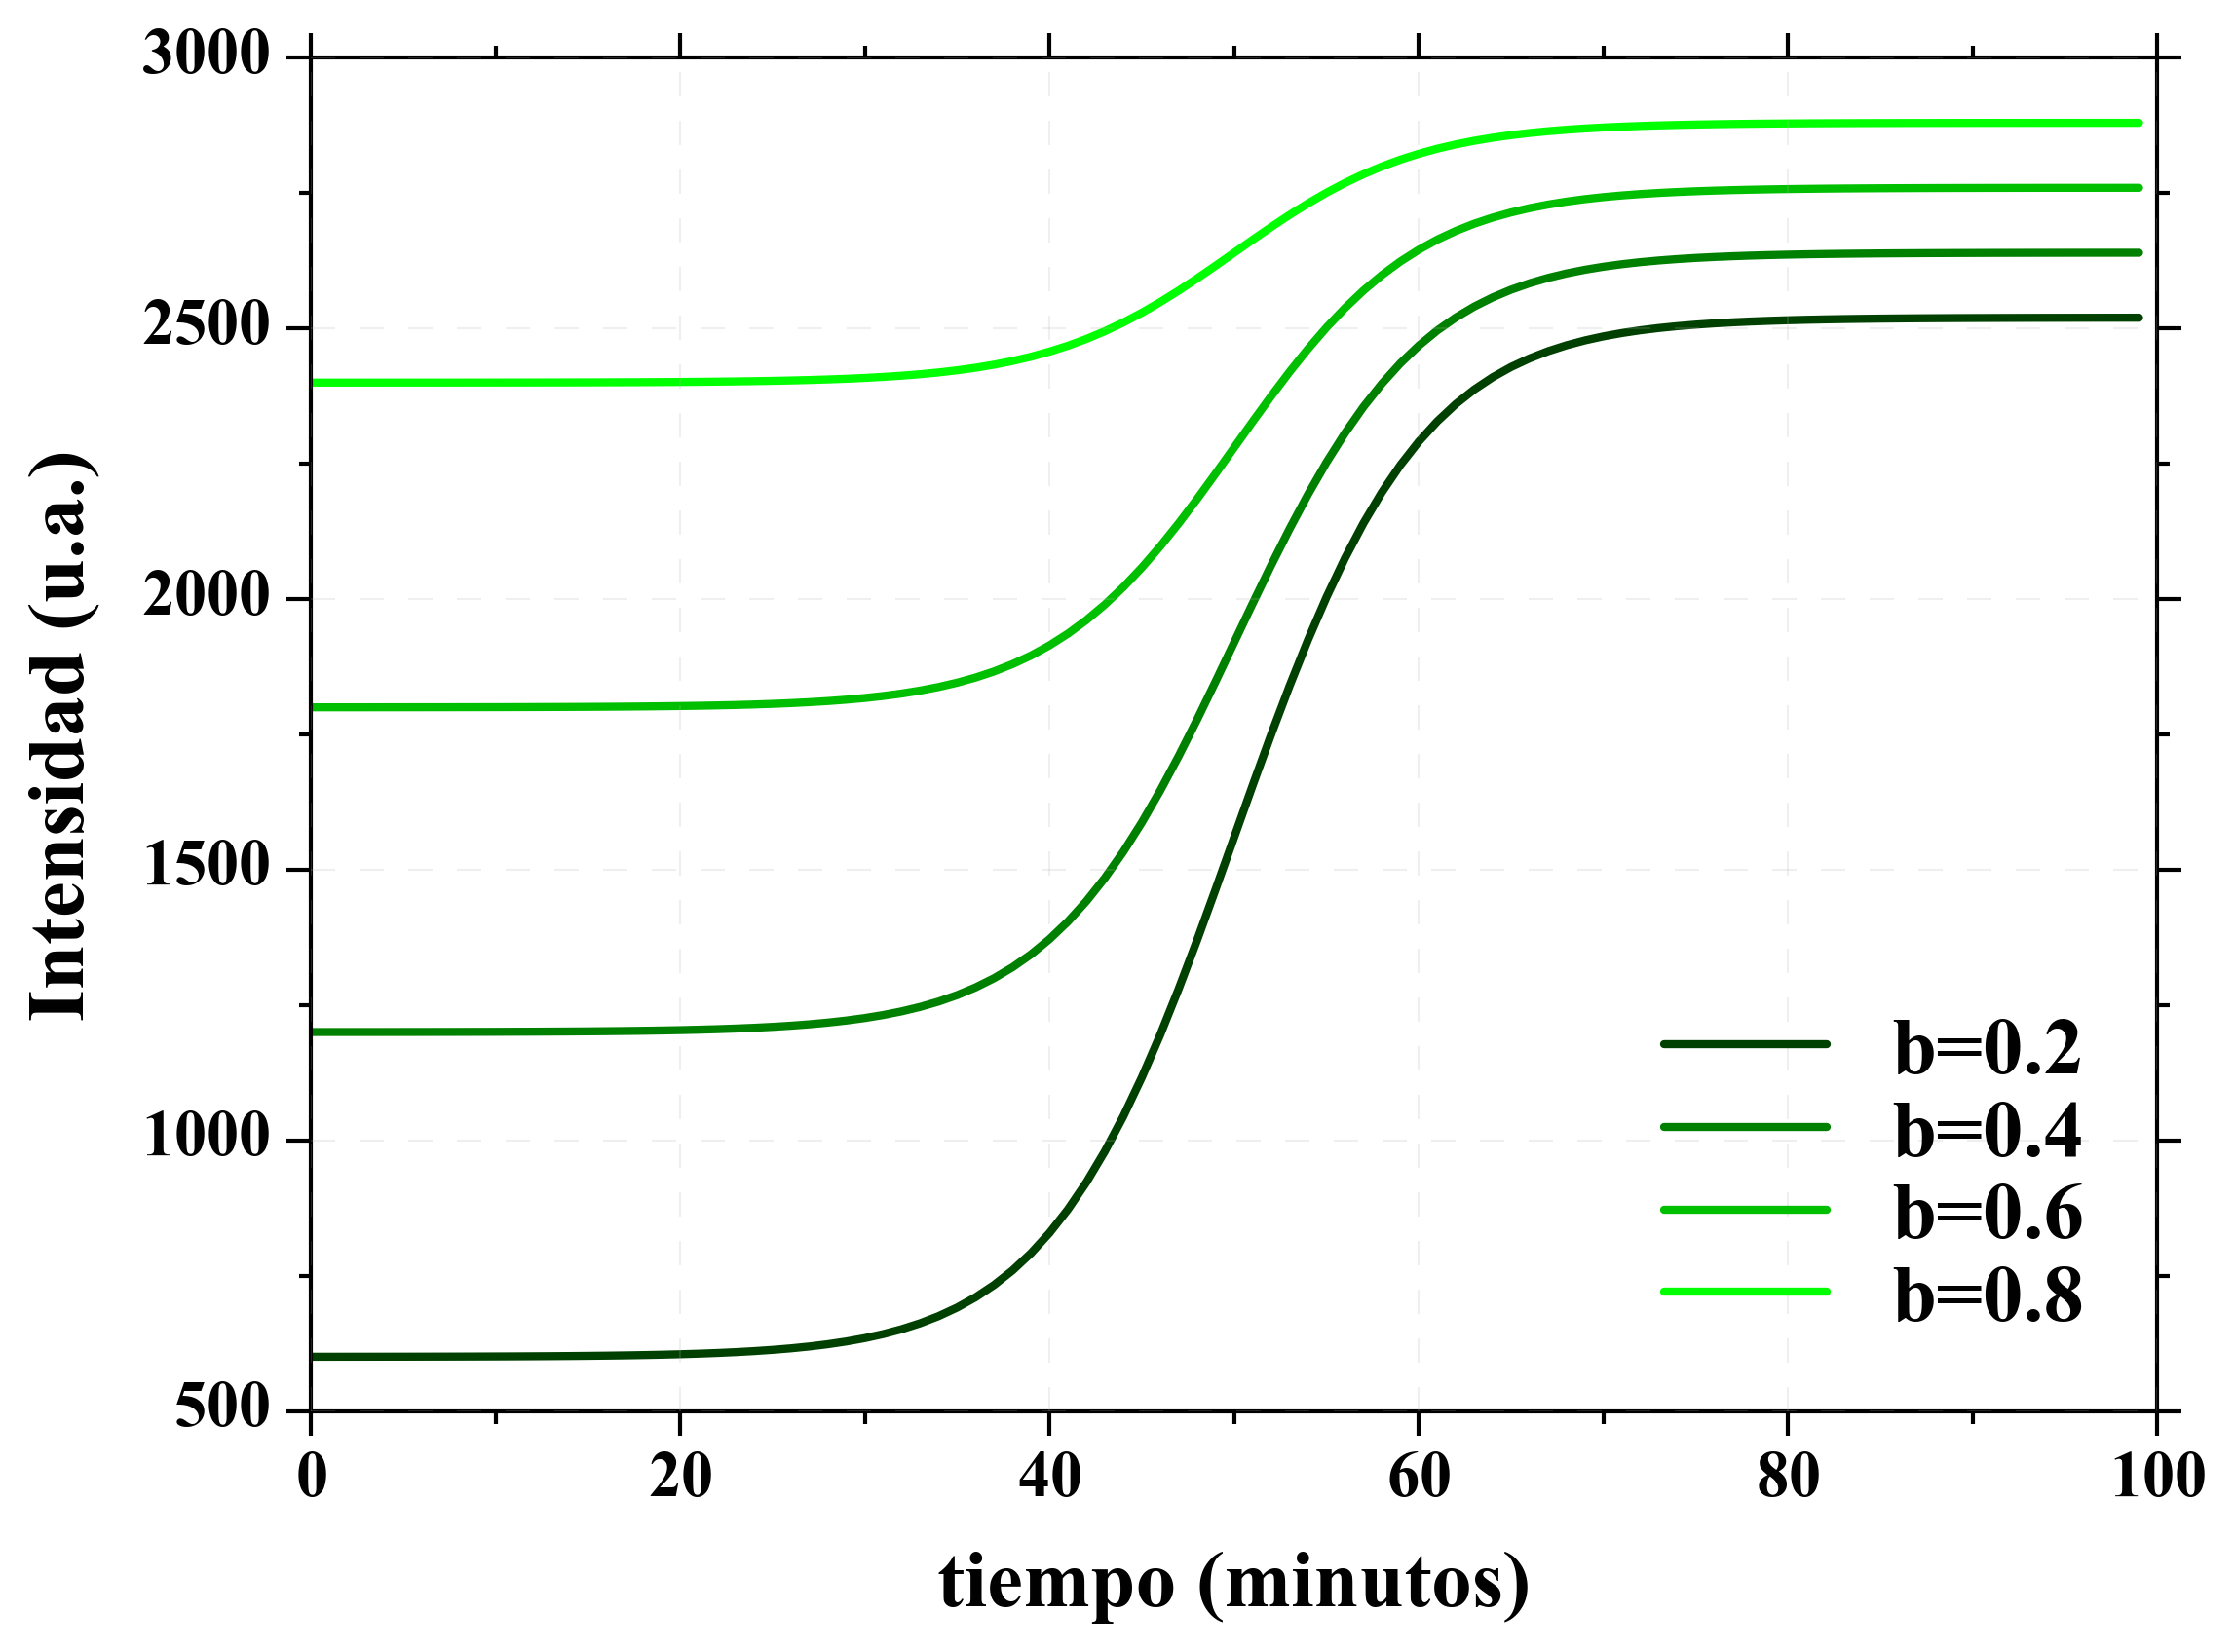
\includegraphics[width=0.6\textwidth]{./img/f_sim.png}
    \caption{Curva de intensidad total de fluorescencia generada a partir de la curva simulada para $m$. Se utilizaron $b_M C = 3000$, mientras que para el valor de $b$ se realizó un barrido entre $0.2$ y $0.8$.}
    \label{fig:f_sim}
\end{figure}

En la figura \ref{fig:f_sim} pueden destacarse algunas características clave de los parámetros. En primer lugar, y como se mencionó previamente, $C b_M$ sirve como parámetro de escala para la intensidad total. Por otro lado, considerando que $b$ muestra la relación entre los brillos de ambos estados del sensor, no nos debe sorprender que cuanto más se aleje de la unidad, mayor será la variación de intensidad de fluorescencia. Además, los distintos valores de $b$ producen distintos valores iniciales y finales de intensidad total. Este hecho sería distinto si el clivaje del sensor fuese del $100\%$.

Podemos apreciar que la anisotropía y la intensidad total de fluorescencia representan un cambio de variables de los observables experimentales que son $I_{\parallel}$ e $I_{\perp}$ a través de la ecuación \ref{eq:anisotropia} y su denominador $I_T = I_{\parallel} +2 I_{\perp}$. Entonces, es posible trabajar sobre cualquiera de las dos, o alguna combinación, para obtener información sobre los parámetros importantes y el estado del ensamble de fluoróforos. Utilizando las relaciones mencionadas, podemos despejar $I_{\parallel}$ e $I_{\perp}$ en función de los parámetros buscados

\begin{align}
    I_{\parallel} &= (\alpha_{\parallel} m + \beta_{\parallel}) \frac{2}{3}Cb_M \label{eq:Int_par}\\
    I_{\perp} &= (\alpha_{\perp} m + \beta_{\perp}) \frac{1}{3} Cb_M,\label{eq:Int_per}
\end{align}

\noindent donde

\begin{multicols}{1}

\begin{align}
    \alpha_{\parallel} & = (r_M + 1/2) - (r_D + 1/2) b\\
    \alpha_{\perp}     & = (1 - r_M) - (1 - r_D) b
\end{align}

\begin{align}
    \beta{\parallel}   & = (r_D + 1/2) b\\
    \beta{\perp}       & = (1 - r_D) b.
\end{align}

\end{multicols}

Habiendo hallado las expresiones matemáticas que describen a $I_{\parallel}$ e $I_{\perp}$ en función de los parámetros y el estado del ensamble, podemos graficar las curvas correspondientes a estas intensidades a partir de la simulación realizada. Dichos gráficos se presentan en la figura \ref{fig:Ints_sim}.

\begin{figure}
\centering
    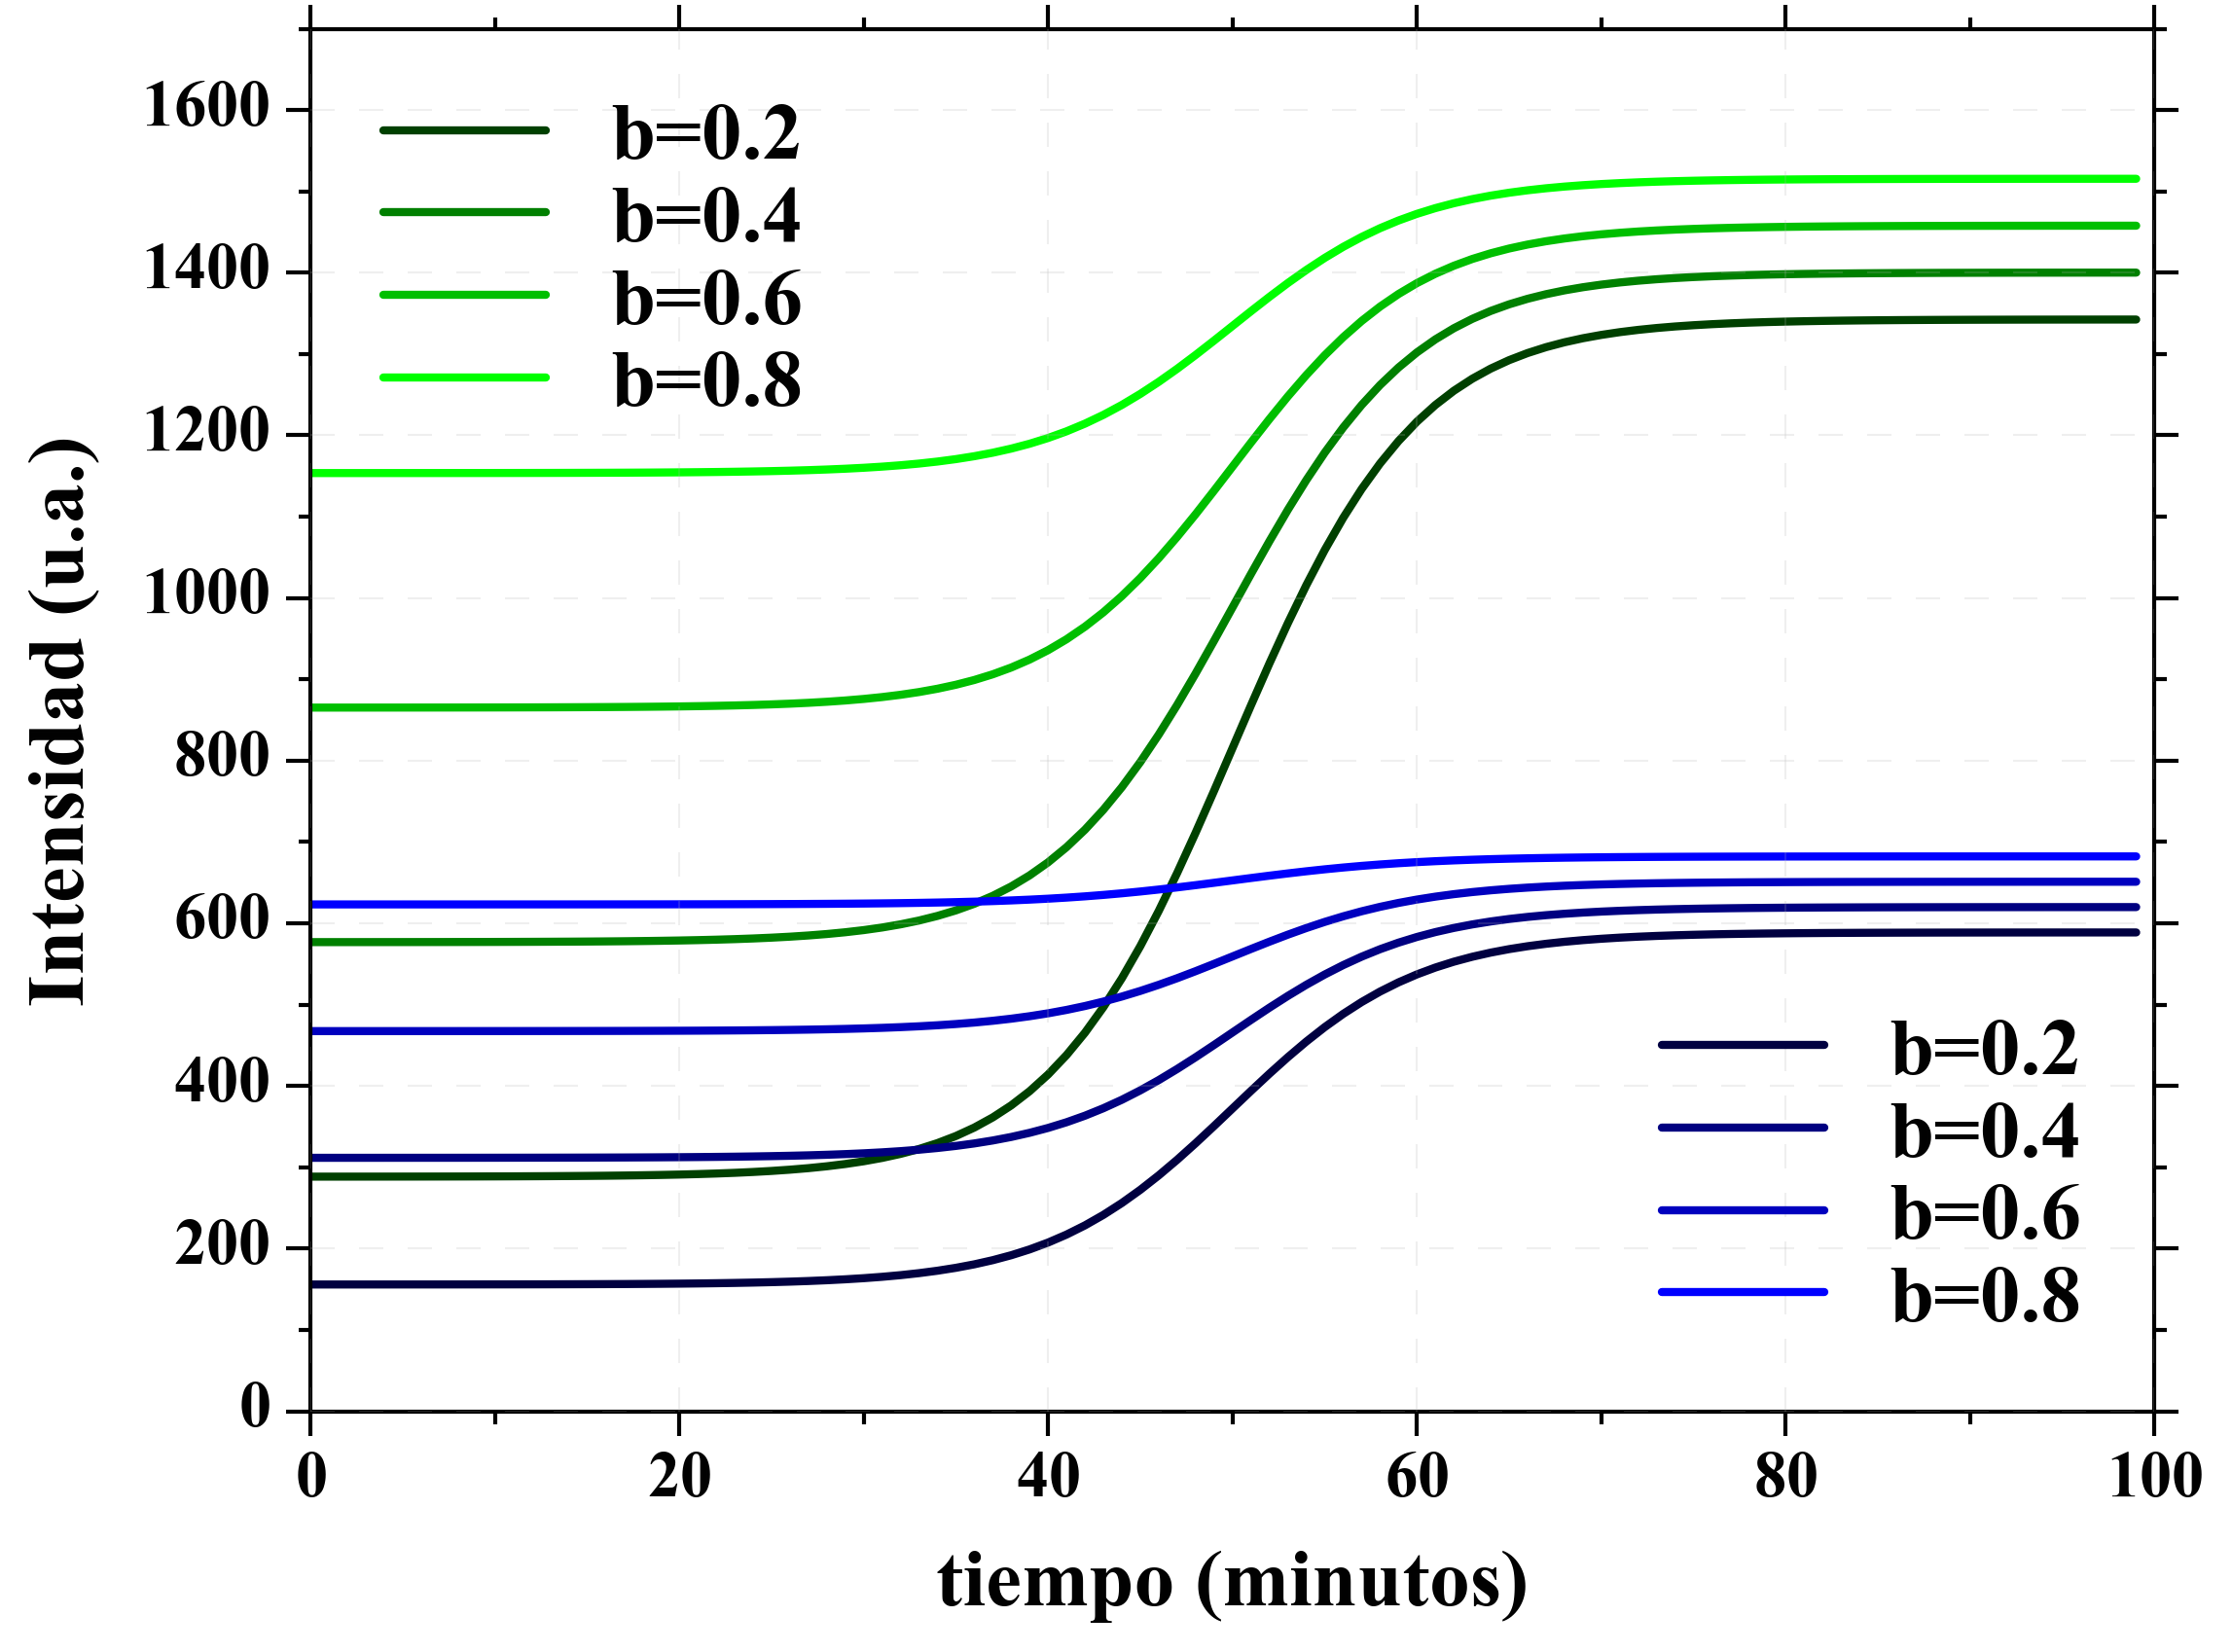
\includegraphics[width=0.6\textwidth]{./img/Ints_sim.png}
    \caption{Curvas de $I_{\parallel}$ e $I_{\perp}$ generadas a partir de la curva simulada para $m$. Se utilizaron los parámetros definidos previamente, a saber, $b_M C = 3000$, $r_D=0.221$ y $r_M=0.303$, mientras que para el valor de $b$ se realizó un barrido entre $0.2$ y $0.8$.}
    \label{fig:Ints_sim}
\end{figure}


%%%%%%%%%%%%%%%%%%%%%%%%%%%%%%%%%%%
\section{Transformación de los Observables Fotofísicos}

A continuación, podemos utilizar las expresiones matemáticas despejadas para transformar los datos simulados y probar así la validez de estos métodos para recuperar información sobre el estado del ensamble de fluoróforos, así como también sus parámetros característicos. En nuestro experimento mental, teníamos una cubeta con un único tipo de sensor cuya cantidad de fluoróforo se mantenía constante a lo largo del experimento, hecho que se refleja en un valor de $C$ constante. Además, los valores de $r_D$, $r_M$, $b_M$ y $b_D$ son específicos para cada fluoróforo, razón por la cual también deben considerarse globales para esta curva. A diferencia de estos parámetros, la proporción de fluróforos en estado monomérico, $m$, puede tomar un valor distinto para cada instante. Aunque esto implicaría que por cada punto agregado, hay un parámetro adicional para ajustar, se debe notar que también se agregan dos observables experimentales medidos, $I_{\parallel}$ e $I_{\perp}$. Si tenemos en cuenta los 4 parámetros globales ($r_D$, $r_M$, $b$ y $C b_M$) y cada $m$ por cada punto, apreciamos que se necesitan al menos cuatro puntos para poder hallar una solución para el sistema. Es esencial notar que $r_D$, $r_M$, $b$ siguen siendo específicos del fluoróforo utilizado, pero $C b_M$ depende de la cubeta analizada ya que cada cubeta puede tener concentraciones distintas.

Con el objetivo de diseñar y validar el método de ajuste para recuperar los parámetros buscados, se programaron en \textit{Python} (\textit{v. 3.4.4}) los algoritmos necesarios para hallar el mínimo de la función de $\chi ^2$. Esta consiste en minimizar

\begin{equation}
    \chi ^2 = \sum \frac{(Observado - Esperado)^2}{Varianza},
\end{equation}

\noindent donde el $Observado$ y la $Varianza$ se refieren a los valores observados experimentalmente mientras que el $Esperado$ corresponde al valor predicho por la teoría. Luego, los parámetros son ajustados para que la curva teórica se asemeje lo más posible a la observada. %En este caso, se utilizaron las ecuaciones \ref{eq:Int_par} y \ref{eq:Int_per} para ajustar las curvas simuladas.

Previo a proceder con los distintos métodos de transformación, discutamos como evaluaremos una buena transformación. Antes que nada, esta claro que debe minimizar $\chi ^2$ de las curvas ajustadas. En segundo lugar, se evaluará si describe adecuadamente la anisotropía observada mediante el cálculo de la suma de todas las diferencias al cuadrado entre los puntos observados y los ajustados. Además, los parámetros utilizados para generar la curva deberían ser recuperables a partir del ajuste, incluso en presencia de ruido blanco. Esta claro, que si la anisotropía es transformada correctamente, el ruido proveniente de su medición también será observado en las curvas de $m$ obtenidas. Esta fidelidad de la transformación con los datos experimentales permite desentenedrnos de las observaciones experimentales y trabajar con la curva de $m$ como si fuese nuestro observable experimental. %Por último, considerando que nuestro objetivo es obtener información confiable del estado del ensamble de fluoróforos, 


%Previo a proceder con los distintos métodos de ajuste mencionados, discutamos como evaluaremos un buen ajuste. Antes que nada, esta claro que debe minimizar $\chi ^2$ de las curvas ajustadas. En segundo lugar, se evaluará si también describe adecuadamente las curvas que no fueron ajustadas pero se deducen a partir del ajuste. Además, los parámetros utilizados para generar la curva deberían ser recuperables a partir del ajuste, incluso en presencia de ruido blanco. Por último, considerando que nuestro objetivo es obtener información confiable del estado del ensamble de fluoróforos, calcularemos el valor de $\chi ^2$ para la curva de $m$ obtenida, así como también $m$ normalizada.

%Por último, introduciremos un parámetro nuevo que cobrará sentido en el próximo capítulo y es importante que sea ajustado correctamente. Este consiste en calcular el máximo de la derivada temporal de $m$ dividido por $d$ (siendo $d=D/C$), al cual denominaremos $\Delta m/d$. Sin entrar en detalles, dicho parámetro nos da una idea de la actividad enzimática y su máximo determina el máximo de actividad.

%\todo{deberia ser $\Delta m$ pero tal vez no haga falta analizarlo}

Habiendo introducido todos los conceptos necesarios para ajustar la transformación de las curvas experimentales, procedemos a evaluar si los parámetros de las curvas simuladas pueden ser recuperados adecuadamente. Simultáneamente, se analizará si el resto de las curvas son recuperadas adecuadamente a partir de las ajustadas. En principio, y siguiendo con el método descripto usualmente en la bibliografía, se ajustará la anisotropía. Dado que son necesarios dos observables para ajustar como se explicó previamente, también utilizaremos la intensidad total observada.

Con el objetivo de introducir ruido en las mediciones de la misma forma que se vería experimentalmente, se confeccionaron funciones que toman las curvas de intensidades cruzadas simuladas y le agregan ruido gaussiano a cada punto. Luego, se recalculaban las curvas de anisotropía e intensidad total a partir de las curvas con ruido agregado. Esto se hizo de esta forma ya que el observable experimental directo son las intensidades cruzadas, y la propagación a anisotropía e intensidad total del ruido no es lineal. Para estas simulaciones se utilizaron las curvas con $b=0.6$.

Ajustar las curvas de anisotropía e intensidad total simuladas mediante las ecuaciones \ref{eq:AnisotropiaFromParams} y \ref{eq:Int_fromFit} dieron muy buenos resultados, como se puede apreciar en la figura \ref{fig:fit_AnNoisy}.

\begin{figure}
\centering
    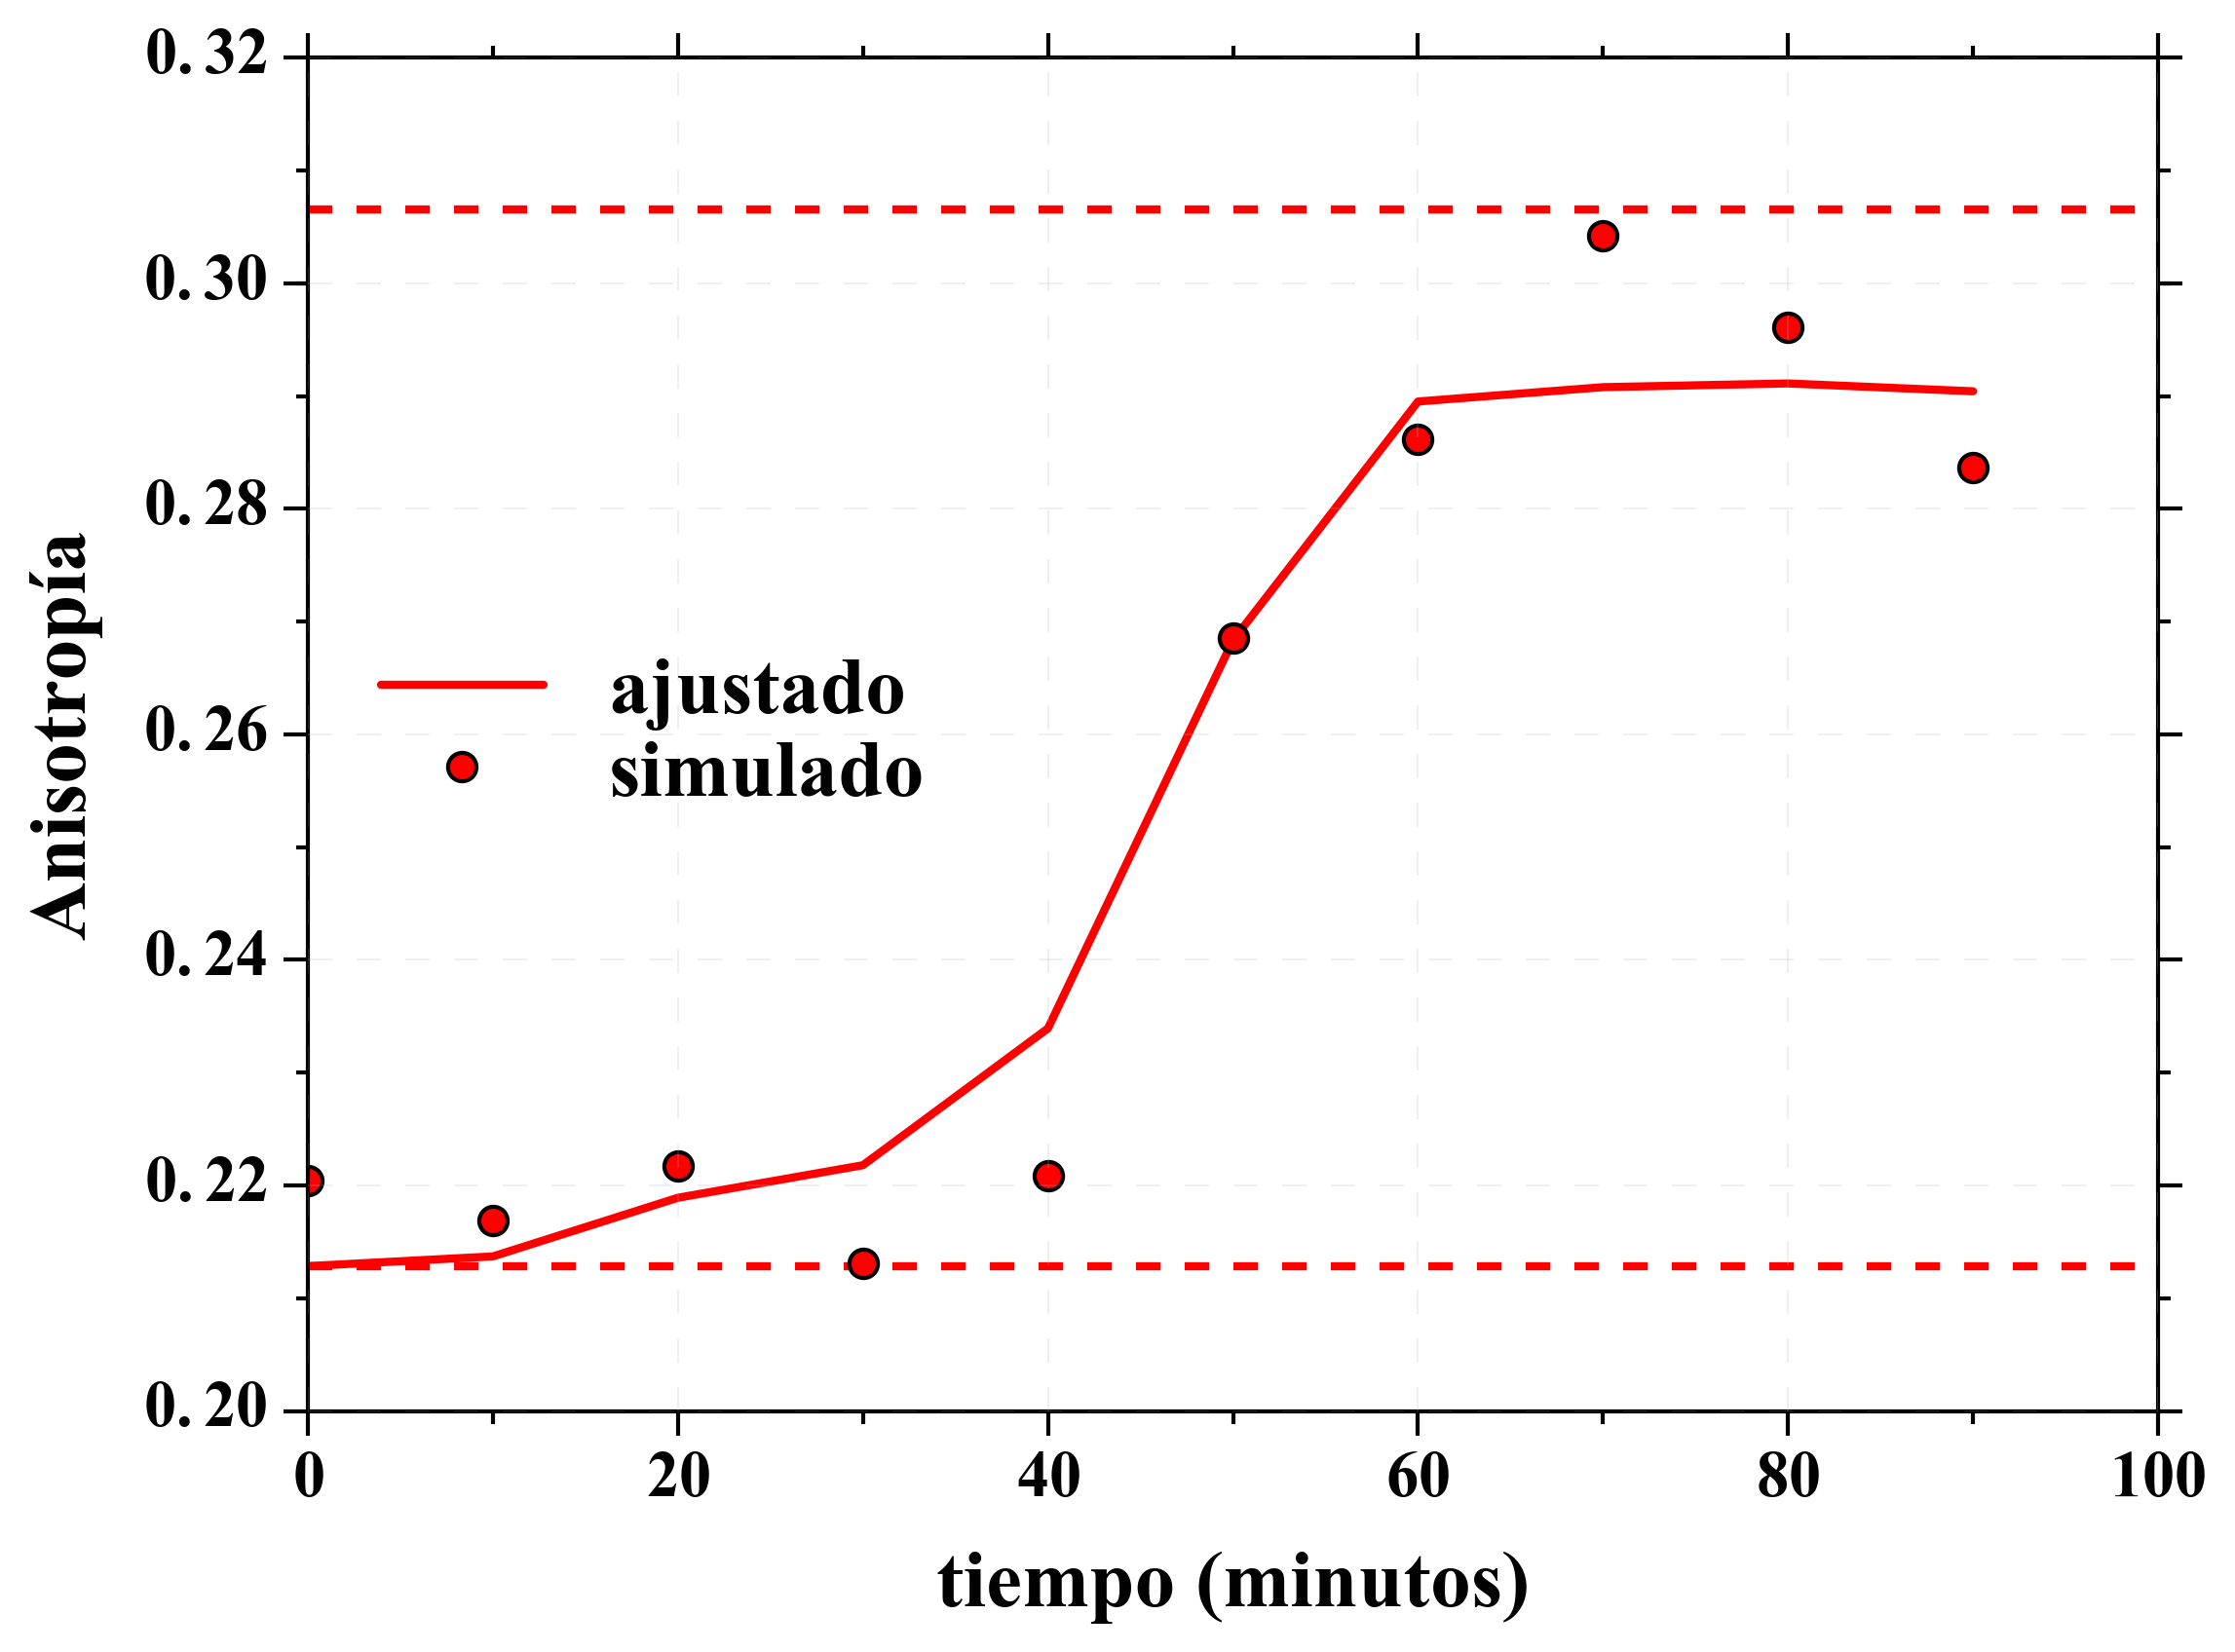
\includegraphics[width=0.5\textwidth]{./img/An_Fit.png}
    \caption{Ajuste de la anisotropía y la intensidad total mediante las ecuaciones \ref{eq:AnisotropiaFromParams} y \ref{eq:Int_fromFit}. Puede apreciarse que el ajuste no recupera de manera fiel los valores de anisotropía, pero promedia el ruido agregado.}
    \label{fig:fit_AnNoisy}
\end{figure}

Dado que experimentalmente se observan $I_{\parallel}$ e y $I_{\perp}$, es buena práctica trabajar directamente con estos observables para evitar propagar sus errores a anisotropía. Se procedió a ajustar dichas curvas simuladas utilizando las ecuaciones \ref{eq:Int_par} y \ref{eq:Int_per}. En la imagen \ref{fig:fit_Icrossed} se presenta un ejemplo de dicho ajuste.

\begin{figure}
\centering
    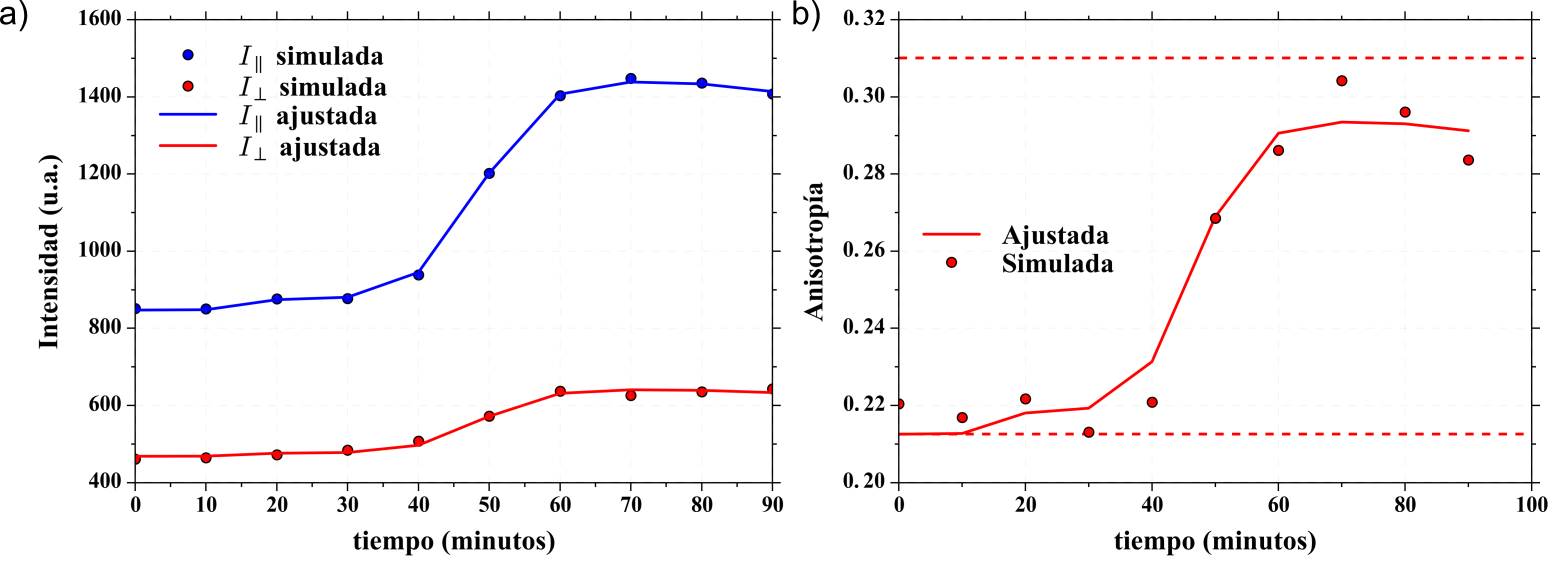
\includegraphics[width=0.9\textwidth]{./img/AjusteInts.png}
    \caption{Ajuste de las intensidades cruzadas mediante las ecuaciones \ref{eq:Int_par} y \ref{eq:Int_per}. \textbf{a)} Gráfico de las intensidades cruzadas ajustadas (trazo continuo) y los datos simulados (círculos). \textbf{b)} Gráfico de la anisotropía ajustada (trazo continuo) superpuesto con los datos simulados de anisotropía (círculos). Puede apreciarse que el ajuste no recupera de manera fiel los valores de anisotropía, pero promedia el ruido agregado.}
    \label{fig:fit_Icrossed}
\end{figure}

Por último, considerando que no se necesita conocer el parámetro de escala se procedió a ajustar las curvas correspondientes a las intensidades cruzadas normalizadas por la intensidad total. Este ajuste tiene la particularidad de que $C b_M$ se cancela en las expresiones a ajustar. Se presenta en la figura \ref{fig:Int_r_Fit} las curvas correspondientes al ajuste y la curva de anisotropía obtenida a partir de este.

\begin{figure}
\centering
    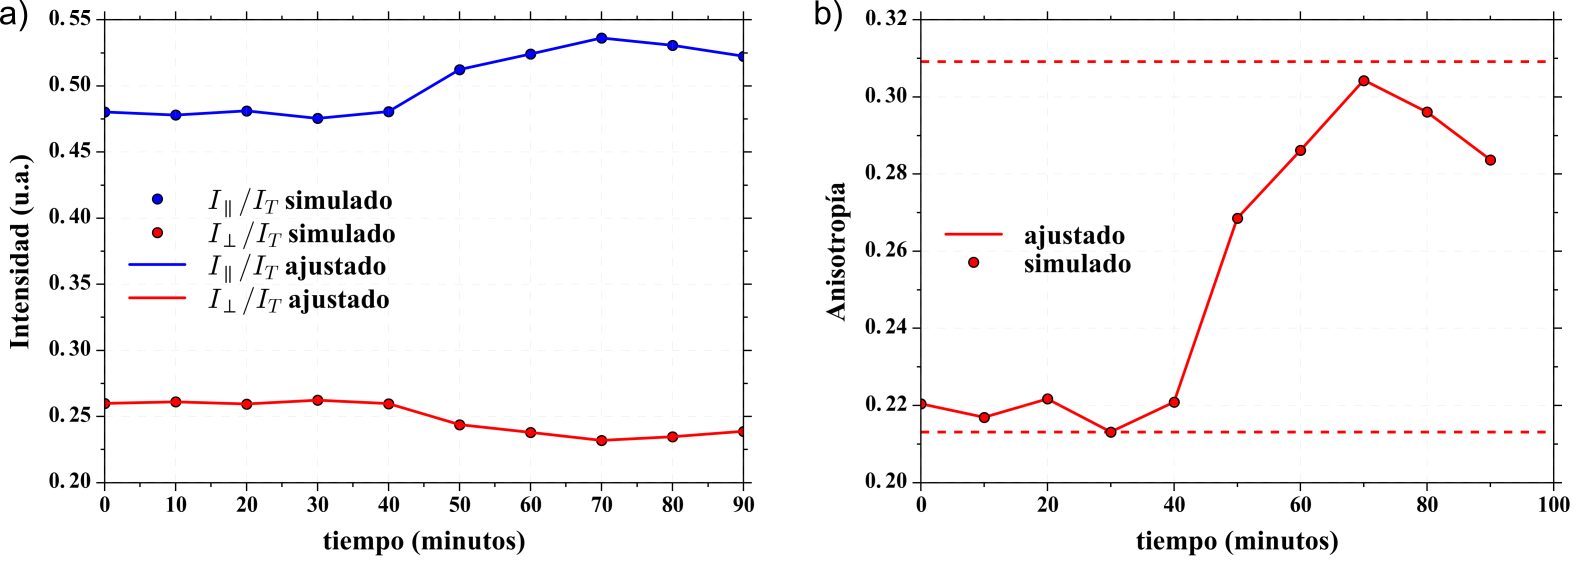
\includegraphics[width=0.9\textwidth]{./img/Ajuste_Int_r.png}
    \caption{Ajuste de las intensidades cruzadas normalizadas. \textbf{a)} Se graficaron las curvas correspondientesa los ajustes de las intensidades cruzadas normalizadas superpuestas con los datos experimentales. \textbf{b)} Se graficó la curva de anisotropía obtenida a partir del ajuste superpuesta con los datos experimentales. Puede apreciarse que el ajuste recupera de manera fiel los valores de anisotropía.}
    \label{fig:Int_r_Fit}
\end{figure}

Habiendo ajustado todas las curvas simuladas, podemos analizar que tan bien fueron reproducidos los parámetros del ajuste. En la figura \ref{fig:fit_Params} se presentan gráficos de los valores recuperados para los parámetros utilizando los distintos métodos. Puede apreciarse una elevada similitud entre ajustar la anisotropía y la intensidad total o las intensidades cruzadas. Por otro lado, la mayor diferencia radica en ajustar las intensidades cruzadas normalizadas. Se debe destacar que este último método no siempre devuelve los parámetros correctamente ajustados.

\begin{figure}
\centering
    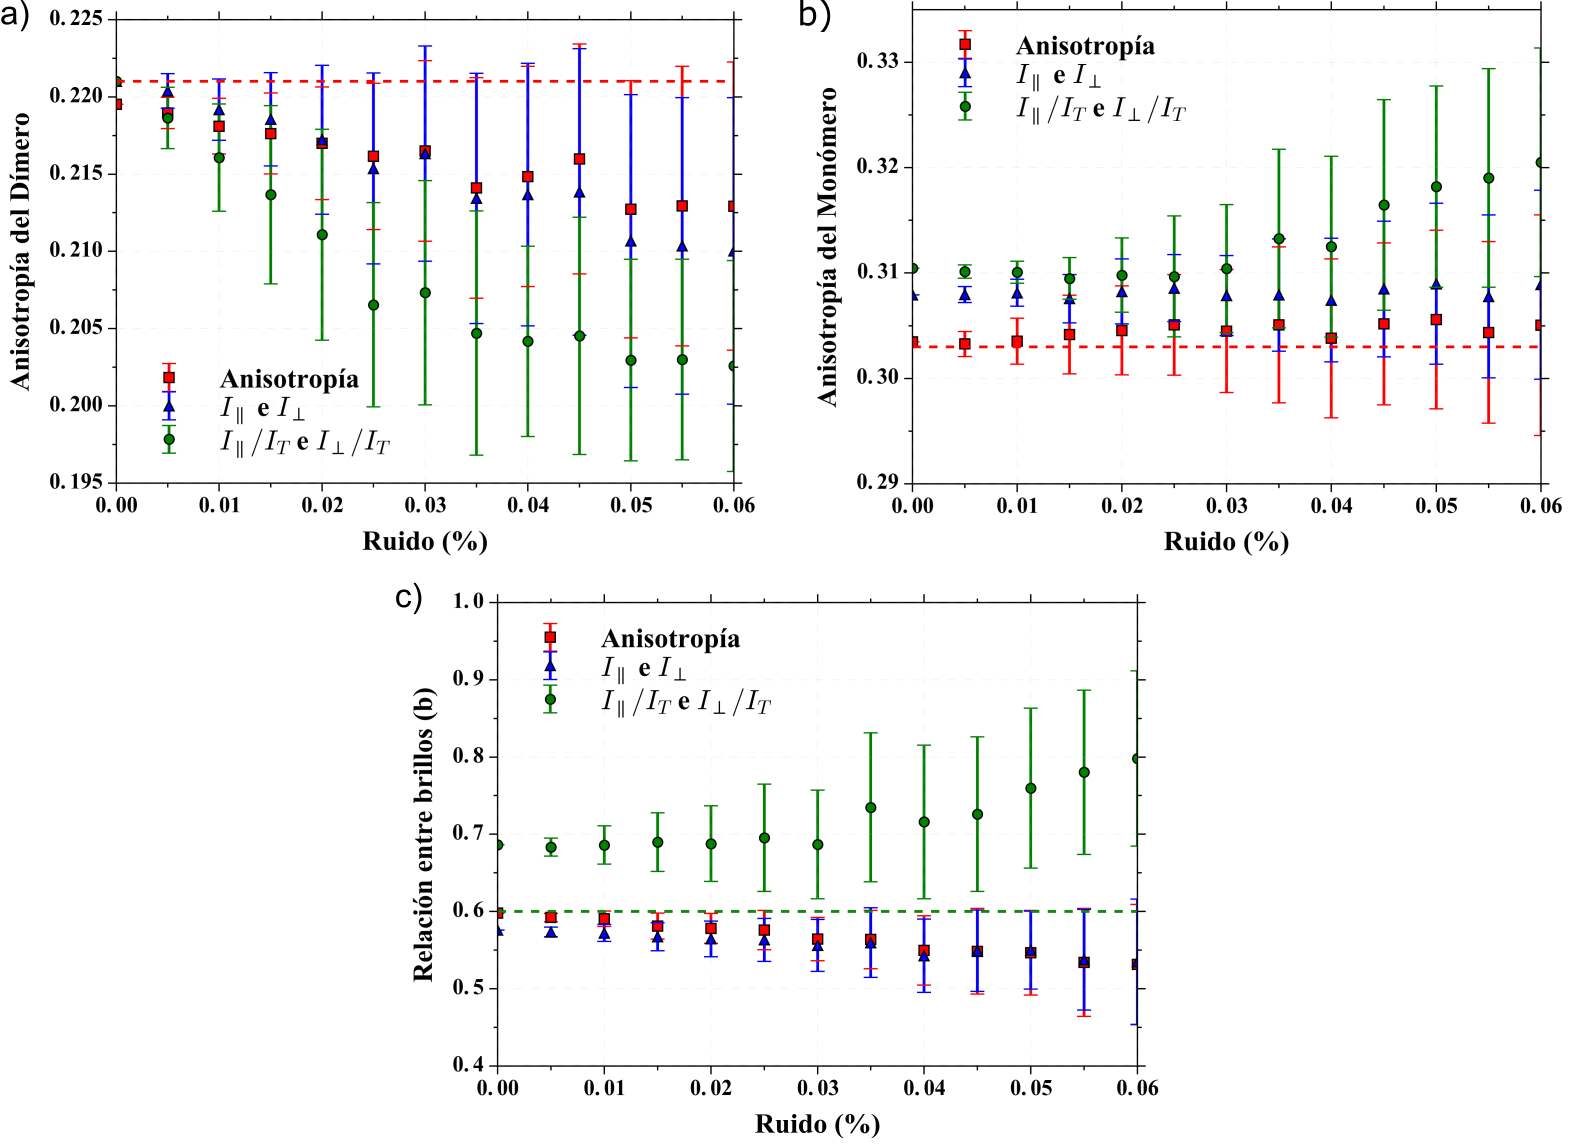
\includegraphics[width=0.9\textwidth]{./img/Ajustes_Params.png}
    \caption{Análisis de parámetros obtenidos a partir de los distintos ajustes. \textbf{a)} Se presentan los valores obtenidos para la anisotropía del Dímero. \textbf{b)} Se presentan los valores obtenidos para la anisotropía del Monómero. \textbf{c)} Se presentan los valores obtenidos para la relación entre intensidades.}
    \label{fig:fit_Params}
\end{figure}

Por otro lado, si observamos la semejanza entre las curvas de anisotropía obtenidas a partir de los parámetros ajustados y la anisotropía generada a partir de la simulación con ruido, podemos apreciar que ajustando las curvas de intensidades cruzadas normalizadas es considerablemente más preciso. En la figura \ref{fig:Ajuste_chi_a} se presenta un gráfico de la suma cuadrática de la diferencia entre los puntos estimados y los simulados para mostrar la afirmación. 
\begin{figure}
\centering
    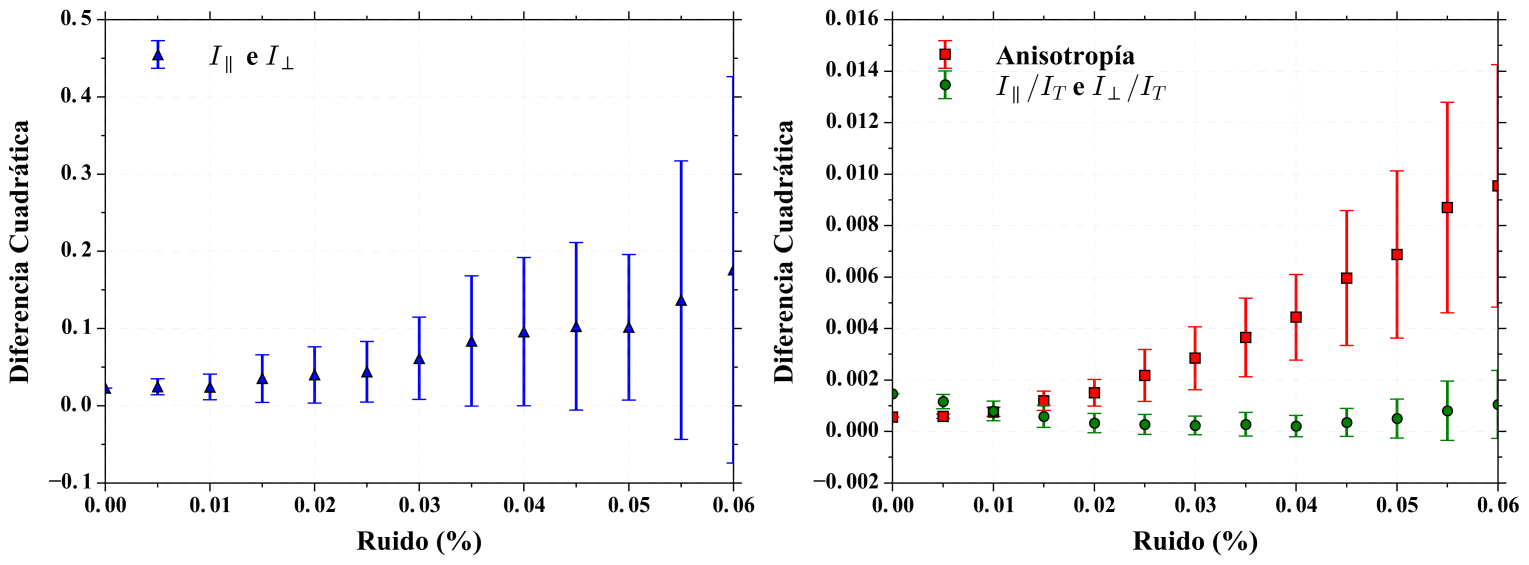
\includegraphics[width=0.9\textwidth]{./img/Ajuste_chi_a.png}
    \caption{Gráfico de la suma cuadrática de la diferencia entre los puntos simulados y los obtenidos a partir del ajuste de los parámetros para la anisotropía. Se graficaron por separado para apreciar la diferencia en orden de magnitud.}
    \label{fig:Ajuste_chi_a}
\end{figure}

A partir de estos análisis se deduce que el ajuste de las intensidades cruzadas normalizadas es fiel al ajuste de la anisotropía, incluso cuando no es el mejor método para obtener el valor de los parámetros. Esto último nos conduce a pensar que ajustar las intensidades cruzadas normalizadas transforma de manera fiel los observables fotofísicos en una curva de proporción de sensor en estado monomérico (ver figura \ref{fig:todos_ms}). De esta forma, uno puede transformar los observables experimentales mediante este método y puede asegurarse que toda la información se verá plasmada en una curva que describe el estado del ensamble de fluoróforos con el mismo ruido que la curva observada experimentalmente. Simultáneamente, este método presenta una mejora teórica al cancelar el parámetro de escala, que varía con cada cubeta.

\begin{figure}
\centering
    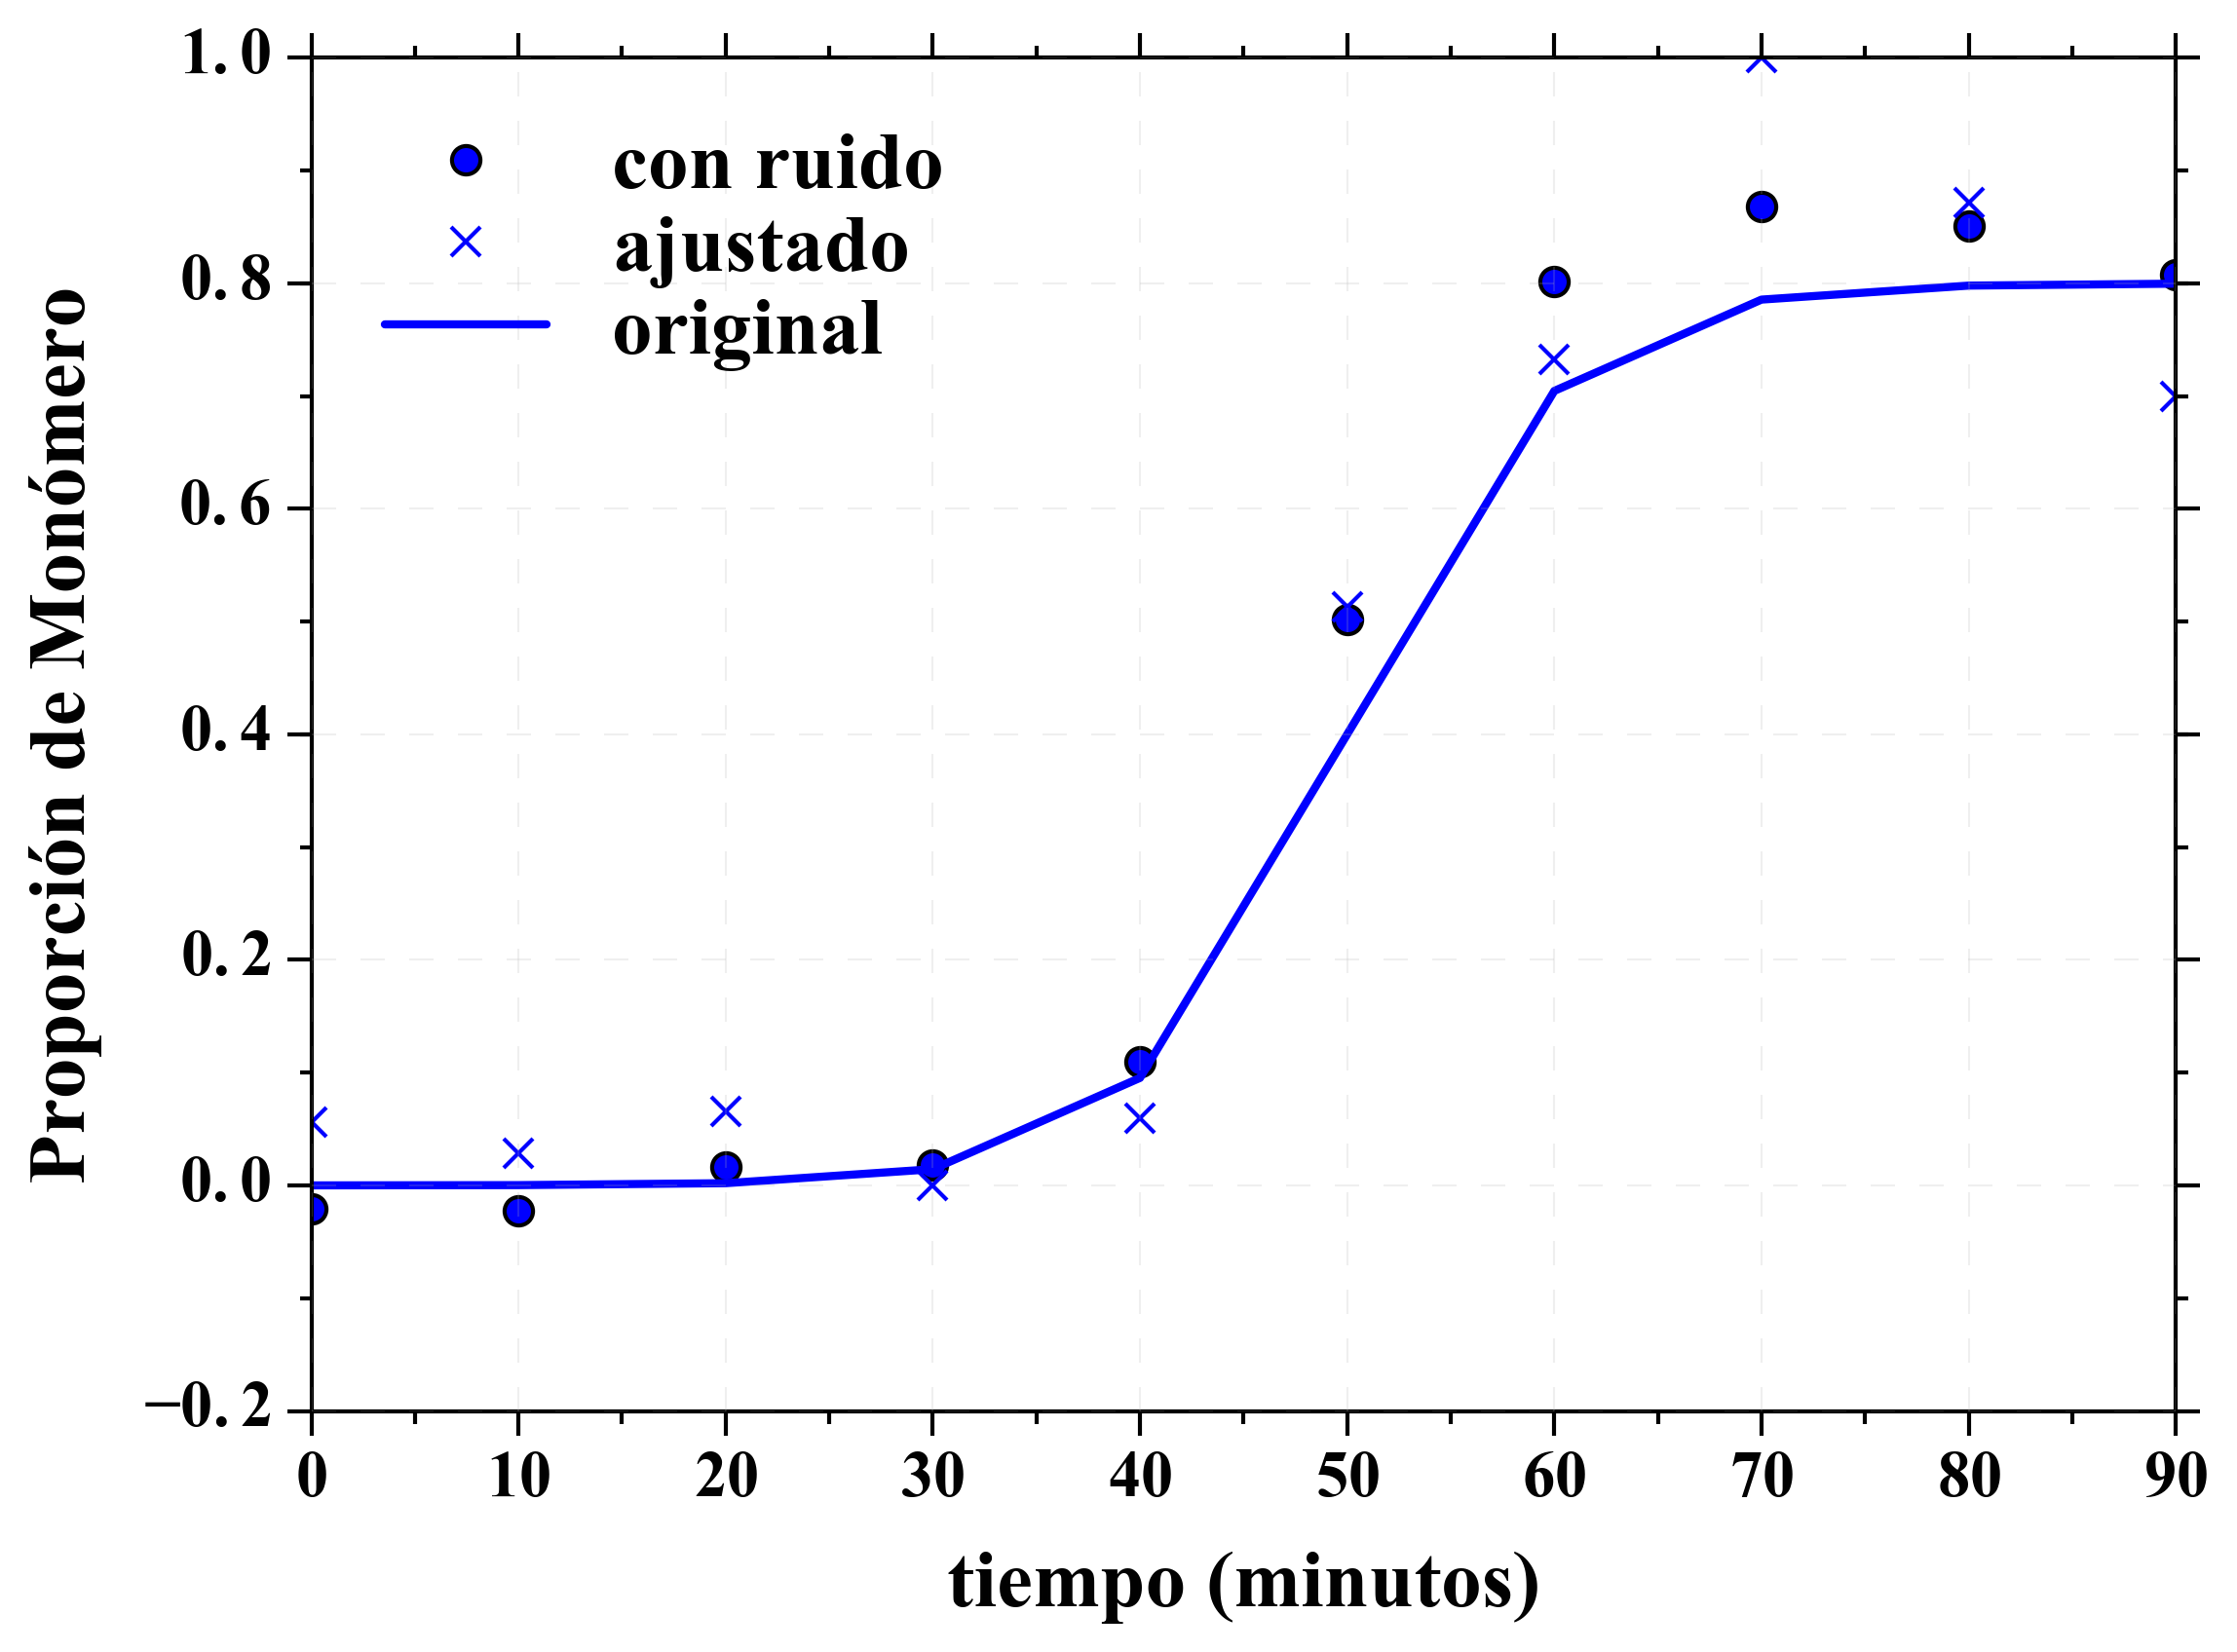
\includegraphics[width=0.5\textwidth]{./img/todos_ms.png}
    \caption{Se superpusieron los gráficos de la curva de proporción de fluoróforo simulada originalmente con sus versiones simuladas con ruido de 3$\%$ y su ajuste. Puede apreciarse una elevada similitud entre los valores obtenidos del ajuste y su contraparte simulada con ruido.}
    \label{fig:todos_ms}
\end{figure}

 %En los casos ideales, este ajuste es capaz de reproducir fielmente los parámetros introducidos, mientras que en la figura \ref{fig:chis} se presenta el corrimiento de $\chi ^2$ a medida que aumenta el ruido en las curvas analizadas.

%En la figura \ref{chis} se presenta una superposición de los valores de $\chi ^2$ obtenidos con cada método de ajuste. Puede apreciarse la ventaja que ajustar las intensidades cruzadas tiene sobre ajustar la anisotropía y la intensidad total. Por lo que se concluye que ajustar sobre los observables experimentales es más robusto que trabajar sobre la señal de anisotropía e intensidad total que se calculan a partir de los observables.


%\todo{Esto es viejo}

%De todas formas, este método produjo resultados pobres al aplicarse a los datos experimentales. Esto se debe principalmente al origen de ruido subyacente en los datos experimentales.

%En la figura \ref{fig:fit_ICrossed_exp} se presenta el ajuste sobre las curvas de intensidades cruzadas y la curva de anisotropía que surgen de los parámetros obtenidos mediante el ajuste. Puede apreciarse una diferencia importante entre la anisotropía obtenida experimentalmente y la correspondiente al ajuste. Esta incongruencia puede explicarse si se tiene en cuenta la propagación de errores al momento de traducir las intensidades cruzadas en anisotropía. Los errores relativos al realizar este pasaje son aumentados al menos en un orden de magnitud, disminuyendo considerablemente el valor de este método.

%\todo{la idea de la propagacion se puede pulir un poco mas}

%\todo{Aca iria la img de ajuste de int cruzadas experimental con la anisotropia obtenida}

%Al analizar la fuente del error en el ajuste, apreciamos que los errores se ven amplificados cuando observamos la curva de anisotropía obtenida. En segundo lugar, variaciones en la máscara generada para segmentar la imagen a analizar nos genera curvas de intensidades cruzadas complicadas de ajustar. Sin embargo, si normalizamos las intensidades obtenidas respecto de la intensidad total podemos, no solo desentendernos del parámetro de escala, sino que las curvas de intensidades cruzadas normalizadas resultan más suaves al despreciar cualquier defecto en la segmentación de imágenes.

%Se repitieron los estudios realizados sobre el método para ajustar intensidades cruzadas y se observó que, aunque los parámetros no podían ser reproducidos adecuadamente, era posible obtener la curva normalizada de proporción de fluoróforo en estado monomérico y sus parámetros de tiempo de máxima actividad.

%En la imagen \ref{fig:fit_ICrossed_N_exp} se presenta un ajuste sobre las curvas de intensidades cruzadas normalizadas y la curva de anisotropía que se obtiene a partir de los parámetros ajustados. Puede apreciarse que la fidelidad entre ambas curvas de anisotropía es mayor que cuando se ajustaban las curvas de intensidades cruzadas sin normalizar. De esta forma, mostramos que ajustando las intensidades cruzadas normalizadas obtenemos una representación más fiel de la proporción de fluoróforo en estado monomérico.

%Si prestamos especial atención a la forma de la curva, podemos apreciar que la anisotropía calculada se asemeja a la intensidad ajustada, hecho que genera una curva de anisotropía poco fiel.

%\todo{Aca iria la img de ajuste de int cruzadas normalizado experimental con la anisotropia obtenida}

%\todo{Esto es mas viejo}

%En realidad hay 3 casos: ajustar anisotropía y fluorescencia total (no lo hice, aunque lo probé con los datos y no andaba), ajustar $I_{\parallel}$ e $I_{\perp}$ (esta hecho y parece andar bien todo en simulada con ruido, pero fallaba con datos) y, por último, las intensidades cruzadas normalizadas (que parecían andar en todos los casos, excepto a la hora de recuperar $b$ en las simuladas).

%Pensaba presentar las dos de intensidades cruzadas, pero tengo muchas cosas para comparar y mostrar. Lo más importante para mí es mostrar que describe bien intensidades cruzadas y anisotropía. Pero después puedo mostrar por cuanto le erra a cada parámetro (gráficos). Y ni hablar de ir variando la proporción inicial y final a la que llega. Todo esto con el método que me dijiste la última vez de dejar libre las anisotropías en el rango que veo experimental, después estaba la posibilidad de fijarlo en cada curva al que mido ahí.

%Para simular el ruido, lo que hacía era meterlo en la anisotropía y la fluorescencia total.

%Ajustar intensidades cruzadas parece devolver mejor el parámetro b. Pero cdo vamos a los datos este método no va bien.